%% TODO fix that f is used as frequency and also as arbitrary function f(t) 
%% TODO get rid of the term "response function" for susceptibility

\add{The theoretical chapter starts with a brief review of \textit{electrodynamics of continuous media}. In its customary form without account for spatial dispersion, this topic is treated in every related textbook, so classical linear electrodynamics is introduced in a minimalistic manner.
%, avoiding many relevant topics such as  TODO, which are not essential for the description of metamaterials.  
This serves as a basis for transforming into the so-called Landau-Lifshitz (or, $EDB$) formulation of electrodynamics for spatially-dispersive media, which is elaborated more in detail.}

\section{Electrodynamics of continuous media} 
\subsection{Electromagnetic wave in vacuum} % FIXME
\paragraph{Maxwell equations}  %{{{
In the realm of classical physics, the electromagnetic phenomena are governed by the \textit{Maxwell equations} in the following form.
We assume here that no free charges and no sources of currents are present: 
\begin{equation} \nabla \cdot  \D = 0, \label{eq_me1}\end{equation}  
\begin{equation} \nabla \cdot  \B = 0, \label{eq_me2}\end{equation}  
\begin{equation} \nabla \times \E = -\frac{\partial \B} {\partial t}, \label{eq_me3}\end{equation}  
\begin{equation} \nabla \times \HH =  \frac{\partial \D} {\partial t}, \label{eq_me4}\end{equation}  
where the $\E$ and $\HH$ are the electric and magnetic vector fields, and $\D$ and $\B$ are the electric and magnetic displacements,
 respectively. These two pairs of field and displacement are related in a similar way as a force is related to the deformation. %% TODO Simovski2007 regards the current J as force, and E as the deformation!
 The \textit{constitutive relations} depend on the properties of the medium the wave propagates in, and in vacuum they take the simplest possible form:
\begin{equation}		\D = \varepsilon_0	\E, \quad\quad\quad						\B = \mu_0			\HH,				 \label{eq_ce}\end{equation}
the $\varepsilon_0 \approx 8.85\cdot10^{-12}$ F/m being the \textit{vacuum permittivity} and $\mu_0 = 4\pi \cdot 10^{-7} \approx 1.25\cdot10^{-6}$ H/m being the \textit{vacuum permeability}. 
Pages \pageref{starttext}--\pageref{endtext} of this thesis will be concerned with computation, interpretation, and experimental verification of the Eq. (\ref{eq_me1}--\ref{eq_me4}) solutions for specific choices of constitutive equations.
%}}}
\paragraph{Wave equation in vacuum} %{{{
\label{starttext}
The pair of first-order differential equations (\ref{eq_me3}, \ref{eq_me4}) can be converted to a single second-order differential equation. To this end, we apply an extra curl operator $\nabla\times$ from the left, and substituting from one equation into the another, we accumulate two curl operators on the left hand side and two derivatives on the right hand side: 
\begin{equation} \nabla\times (\nabla\times \E) = \nabla\times \left(- \frac{\partial \B} {\partial t}\right) = -\mu_0 \frac{\partial}{\partial t} \left(\nabla\times \HH\right) 
= -\mu_0 \frac{\partial^{2} \D}{\partial t^{2}} = -\mu_0 \varepsilon_0 \frac{\partial^{2} \E}{\partial t^{2}}.  \label{eq_elim}\end{equation}
Using the vector calculus identity
\begin{equation} \nabla\times (\nabla\times \E) \equiv \nabla (\nabla \cdot \E) - \nabla^2 \E, \label{eq_rotrot}\end{equation}
we obtain the \textit{wave equation} for the electric field in vacuum: 
\begin{equation}  \nabla (\nabla \cdot \E) - \nabla^2 \E = -\mu_0 \varepsilon_0 \frac{\partial^{2} \E}{\partial t^{2}}.  \label{eq_wave}\end{equation}
%Note this holds for each component of electric field independently. -- NOT: the divergence is not independent of other components
Starting with Eq. (\ref{eq_me4}) instead of (\ref{eq_me3}), the same result could also be easily obtained for the magnetic field $\HH$.
%% TODO develop why (E, H, k) forms the RIGHT-handed triplet
%}}}
\paragraph{Plane wave} %{{{
The solutions of the linear wave equation (\ref{eq_wave}) can be decomposed as a sum of \textit{harmonic plane waves}, where \textit{harmonic} means that the amplitude depends on the time $t$ as a harmonic function (e.g. $\sin(t)$). As a \textit{plane wave} we denote such a spatial shape of the fields, that is a function of a single  scalar parameter $\kk\cdot\rr$. Assuming the wave propagates with nonzero velocity, also the spatial dependence on  $\kk\cdot\rr$ must be harmonic, and therefore 

Any other complicated shape of the fields can be decomposed into a linear superposition of more such waves and treated separately \cite{jackson1962book}. 

%Linear electrodynamics is often treated with the 
The electromagnetic field will described as a complex exponential, i.e. as a superposition of two waves differing by a mere quarter-period phase shift, one defining the real part, one the imaginary part of the field. In comparison with the intuitive description of a plane wave in terms of a cosine (or sine) function, the complex notation formally simplifies some mathematical operations, e.g. it allows to easily identify the \textit{phase of a wave as} the exponent, when multiplied by $\ii$. 

 

%% TODO add figure: plane wave
Without loss of generality, we define the electric field as a function of time $t$ and position in space $\rr$, corresponding to a plane wave in the complex notation:
\begin{equation} \E(t, \rr) := \E_0\, e^{\ii\omega t - \ii\kk\cdot\rr} \label{eq_pw}\end{equation}
The plane wave is fully characterised by its \textit{amplitude vector} $\E_0$, \textit{angular frequency} $\omega$ and \textit{wave vector} $\kk$. Note that no restrictions were put to the amplitude vector $\E_0$ so far, thus Eq. (\ref{eq_pw}) can describe both \textit{transverse} wave of any polarization, with $\E_0 \perp \kk$, and \textit{longitudinal wave} with $\E_0 || \kk$.

As discussed in the introduction, the time dependence of complex fields with positive evolution in time ($e^{+\ii\omega t}$)  was chosen without any impact on the physical consequences.

%}}}
\paragraph{Dispersion relations in vacuum} %{{{
Only some combinations of ($\E_0, \omega, \kk$) provide a physical solution of the wave equation (\ref{eq_wave}). In vacuum, the allowed solutions can be obtained by first substituting the differential operators by their equivalents for a particular plane wave: %TODO explain
\begin{equation} \nabla \rightarrow -\ii\kk, \quad\quad\quad 
\frac{\partial} {\partial t} \rightarrow \ii\omega, \label{eq_difftok}\end{equation}
so the wave equation (\ref{eq_wave}) can be modified the following way:
$$					\nabla (\nabla \cdot \E) - \nabla^2 \E				  =	-\mu_0 \varepsilon_0 \frac{\partial^{2} \E}{\partial t^{2}},  $$
$$				 -\ii\kk (-\ii\kk \cdot \E)  - (-\ii\kk \cdot -\ii\kk) \E = -\mu_0 \varepsilon_0 (\ii\omega)^2 \E, $$
$$   - \kk (\kk \cdot \E)      +          k^2 \E            = +\mu_0 \varepsilon_0 \omega^{2} \E,  $$
\begin{equation}  T\E            = \frac{\mu_0 \varepsilon_0 \omega^{2}}{k^2} \E.  \label{eq_wavek}\end{equation}
The linear operation $T$ of the left hand side can be geometrically interpreted as taking the transverse component of the field $\E$, that is, perpendicular to the wavevector $\kk$. 
\begin{equation} T\E :=  -\frac{\kk (\kk \cdot \E)}{k^2} + \E     \equiv     - \frac{\kk\times(\kk\times\E)}{k^2} \label{eq_transverse1}\end{equation}
Rewriting it explicitly, we define the \textit{wave-plane projection tensor} that will be useful in the following chapters, too:
\begin{equation} T = \frac{1}{k^2} 
\left(\begin{array}{ccc} 
	k_y^2+k_z^2  	& -k_x k_y 		& -k_x k_z \\ 
	-k_y k_x 		& k_x^2+k_z^2	& -k_y k_z \\ 
	-k_z k_x 		& -k_z k_y		& k_x^2+k_y^2
	\end{array} \right) 
\text{ or equivalently, }
T_{ij} = - \frac{k_i k_j}{k^2} + \delta_{ij} .  \label{eq_transverse2}\end{equation}
The solutions of Eq. (\ref{eq_wavek}) for a harmonic plane wave in vacuum divide into two groups: % TODO add reference that there is no other oslutino
\begin{enumerate}
 \item{\textit{Transverse electromagnetic waves}, with the electric field and wave vector being perpendicular, i.e. $(\kk \cdot \E) = 0$ and thus $T\E = \E$. Therefore, the \textit{dispersion relation} for a transverse plane wave in vacuum is linear:
\begin{equation} k~= \sqrt{\mu_0 \varepsilon_0}\; \omega = \frac{\omega}{c}, \label{eq_dispeq_vac}\end{equation}
where we defined the \textit{speed of light} $c := \frac{1}{\sqrt{\mu_0 \varepsilon_0}}$. The corresponding solution is plot in Fig. \ref{fg_dcvac}, independent of the orientation of the wavevector $\kk$.
} 
 \item{\textit{Longitudinal electromagnetic waves}, with $\kk\,|| \pm \E$ and $T\E = 0$, require the right side of Eq. \ref{eq_wavek} to be zero. In vacuum, there is no such a solution, except for a homogeneous static electric field ($k = 0, \omega = 0$), but they will be shown to exist in dispersive media.} 
 \end{enumerate}
 \begin{figure}[t] \caption{Left panel shows the permittivity $\epsrl'$ and permeability $\murl'$ of vacuum being equal to 1; as a result, the dispersion curve for a transverse wave in vacuum forms a straight line in the right panel. As in the case of similar plots later, both axes of the right panel are normalized to an arbitrary frequency of $\omega_0$, because the characteristic curve shapes are independent of the scale.} \label{fg_dcvac} \centering  %% TODO refto
	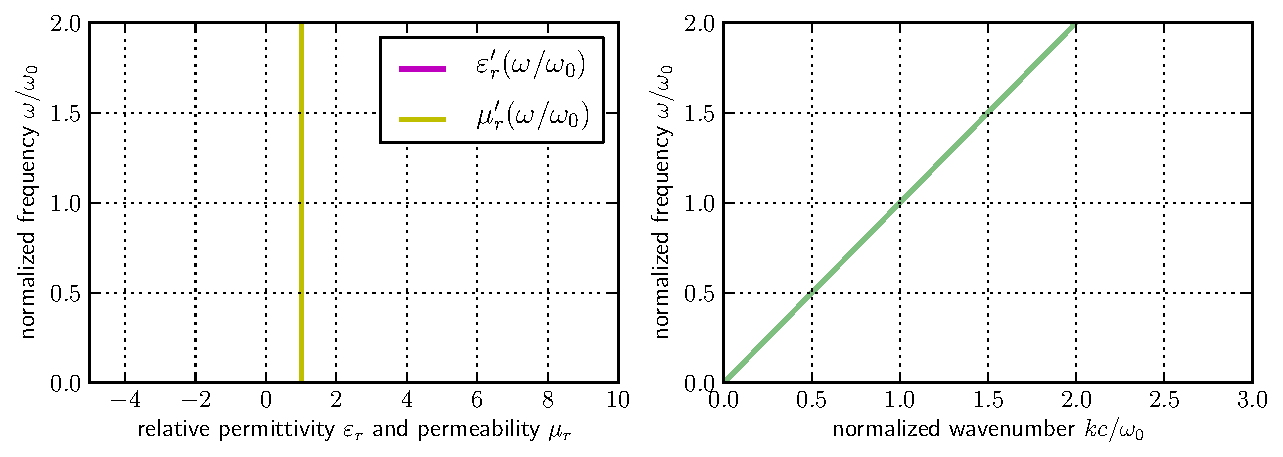
\includegraphics[width=17cm]{img/dispersion_landau_lifshitz/dispersion_vacuum.pdf}
\end{figure}
%}}}

\subsection{Local response of media to the electromagnetic field} \label{loc_response_of_media}
\paragraph{Local response definition} \label{subsection_local_resp} %{{{
In the whole chapter, we expect the medium properties to be time-invariant, linear, and homogeneous (i.e. independent of time, field amplitude and position in space, respectively). 
In this section, we focus on the special case when the medium response in point $\rr$ is not influenced by the electric field in any other point $\brho \neq \rr$. The medium is then said to be \textit{local}. 
For most media found in nature, this approximation is very close to reality and thus numerous electrodynamics textbooks tend to omit the nonlocal effects. 
However using this local theory to a wave propagating through periodic structures has a priori no justification and may lead to completely wrong results. The local theory presented here will serve as a basis for the nonlocal theory developed in following chapters.
% Applying the more familiar local electrodynamics to these structures is a mistake common to many papers. While the local theory is mathematically consistent, it predicts unusual spectral shapes and does not allow their further physical interpretation.

When an electric field $\E$ is applied, the medium responds by a change of the electric displacement $\D$ in a way that is characteristic for it. 
The immediate response of vacuum from the right side of the constitutive equations (\ref{eq_ce}) remains unchanged, but the response of the matter adds a new term called \textit{electric polarisation}. The polarisation is not instantaneous, so it is generally expressed as a convolution of the \textit{electric susceptibility} $\chi_e$ with the values of electric field in the previous time $\tau$:
\begin{equation} \D(t,\rr) = \varepsilon_0 \E(t,\rr) + \varepsilon_0 \int_{-\infty}^{t}\chi_e(t-\tau)\, \E(\tau,\rr)\,\mbox{d}\tau. \label{eq_loc_chi_convol}\end{equation}
Assume that a harmonic plane wave propagates through the medium, so $\E(t, \rr) := \E_0 \, e^{\ii\omega t - \ii\kk\cdot\rr}$, as given by Eq. (\ref{eq_pw}). This can be inserted in the above equation:
\begin{equation} \D(t,\rr) = \varepsilon_0 \E_0 \, e^{\ii\omega t - \ii\kk\cdot\rr} + \varepsilon_0 \int_{-\infty}^{t} \chi_e(t-\tau) \, \E_0 \, e^{\ii\omega \tau - \ii\kk\cdot\rr} \,\mbox{d}\tau. \label{eq_chi_convol_harm}\end{equation}
Substituting $T:=t-\tau$, the exponent can be separated into two parts: one of which factors out of the integral, and the remaining part that turns the convolution into a temporal Fourier transform of the medium response:
$$				 \D(t,\rr) = \varepsilon_0 \E_0 \, e^{\ii\omega t - \ii\kk\cdot\rr} + \varepsilon_0 \int_{-\infty}^{0} \chi_e(T) \, \E_0 \, e^{\ii\omega (t - T) - \ii\kk\cdot\rr} \,\mbox{d}T,$$
$$				 \D(t,\rr) = \varepsilon_0 \E_0 \, e^{\ii\omega t - \ii\kk\cdot\rr} + \varepsilon_0 \left( \int_{-\infty}^{0} \chi_e(T)  \, e^{-\ii\omega T}\,\mbox{d}T  \right) \E_0 \, e^{\ii\omega t - \ii\kk\cdot\rr}.$$
%% NOTE that the Fourier transform is never subject to the sign change, cf. \ref{eq_kkF}
This is nothing but an application of the convolution theorem: convolution in time domain is equivalent to multiplication the in frequency domain.  %% FIXME normalisation by 2pi?
Consequently we may introduce the local \textit{relative permittivity} $\epsrl(\omega)$ as a function of frequency. It is a property of the medium that determines how strong it develops the electric displacement $\D$ in response to a harmonic wave. From Eq. (\ref{eq_ce}) it is clear that in vacuum,  $\epsrl = 1$.
\begin{equation}  \epsrl(\omega) = \left.\frac{\D(t,\rr)}{\varepsilon_0 \E(t,\rr)} \right|_{\E(t, \rr) := 1 + \chi_e(\omega) = \E_0 \, e^{\ii\omega t - \ii\kk\cdot\rr}} = 1 + \int_{-\infty}^{0} e^{-\ii\omega T} \,\chi_e(T) \,\mbox{d}T \label{eq_eps_loc}\end{equation}
%% TODO note that in freq domain this is a complex-valued function, unlike time-domain response; and explain why it is so: that it allows to easily pack in also the information about the phase
%}}}
\paragraph{Response of a harmonic oscillator} \label{chap_lorentzmedia} %{{{
\begin{figure}[t] \caption{\textbf{a)} Illustration of how a simplified medium may respond to an electric field impulse in the shape of Dirac delta function  $E(t) = \delta(t)$. The response is composed from an instantaneous part from vacuum, $\delta(t)$, and from a delayed ringdown of one damped harmonic oscillator, described by $\chi_e(t) := 2\pi \sin(2\pi t)\,e^{-x/2}$; \textbf{b)} The corresponding local permittivity $\epsrl(\omega)$, computed by Fourier transform of the response. Note that the imaginary part of permittivity is negative due to that the material is lossy (absorbs energy) and that the $e^{\ii\omega t}$ convention is used.} \label{fg_oscillator_spectrum} \centering 
	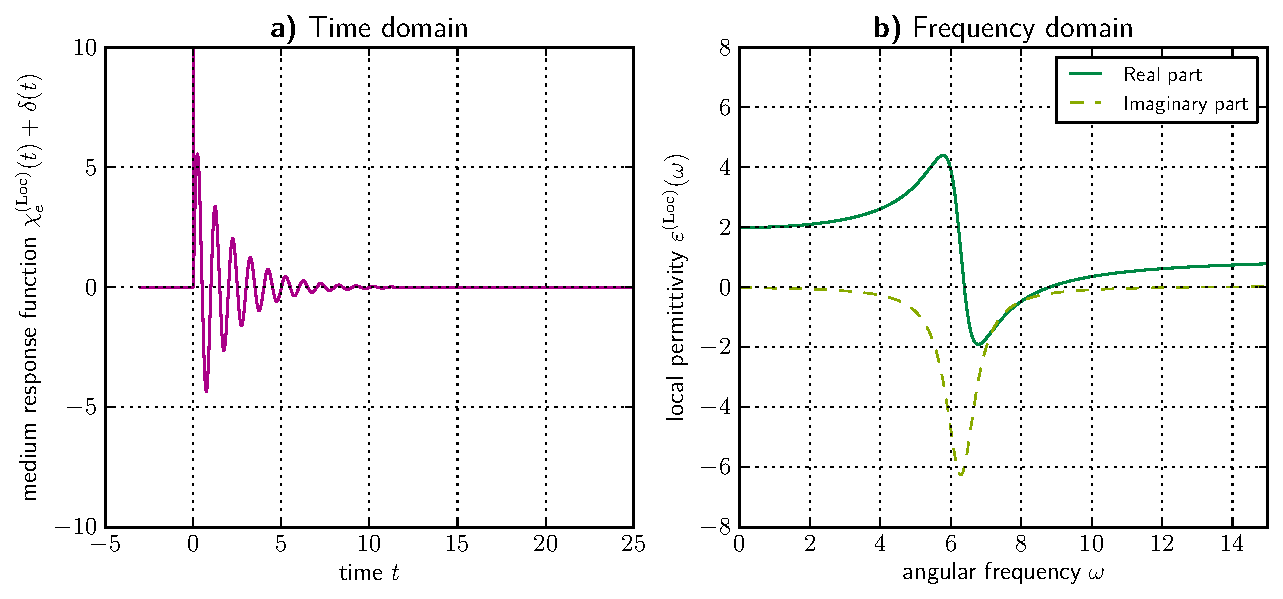
\includegraphics[width=17cm]{img/oscillator_spectrum.pdf}
\end{figure}
The response function $\chi_e(T, \mathbf{R})$ of usual media is composed of different phenomena.  Each of them may react on different time scales, and thus the medium response usually has a relatively complicated shape in the time domain.  However, to a reasonable degree of approximation, each of the contributions can be treated separately, as is demonstrated in the following.

Linear physical systems with an inertial mass, friction force and a restoring force are known as \textit{damped harmonic oscillators}.  This theory applies well to the electrons elastically bound to an atomic nucleus, as well as to the atoms elastically bound to their equilibrium position in the lattice. The molecular rotation can also be modelled as an (possibly overdamped) harmonic oscillator. Even the free electrons in conductive media can fit into the theory of harmonic oscillator provided the restoring force is set to nearly zero. The response of a harmonic oscillator is easy to describe both in time domain and frequency domain, even without the explicit use of the Fourier transform from Eq. (\ref{eq_eps_loc}). The harmonic oscillator model thus becomes a convenient starting point to approximate the response of materials.

A damped harmonic oscillator is described by a second-order differential equation:
\begin{equation} \alpha \frac{\partial^{2} x(t)}{\partial t^{2}} + \beta\frac{\partial x(t)}{\partial t} + \zeta x(t) = f(t). \label{eq_harm_osc}\end{equation}
Provided the driving term on the right hand side  is harmonic $f(t) = e^{+\ii \omega t}$, the system response is also a harmonic function, $x(t) = \chi(\omega) e^{+\ii \omega t}$. The differential equation (\ref{eq_harm_osc}) can be easily solved to show that the complex amplitude of the driven oscillations, $\chi(\omega)$, depends on the angular frequency and on the parameters $\alpha$, $\beta$ and $\zeta$ in the following way:
\begin{equation} \chi(\omega) \equiv \frac{x(t)}{f(t)} = \frac{1}{\zeta-\alpha\omega^{2} + \ii\omega\beta}  = \frac{\alpha^{-1}}{\frac{\zeta}{\alpha}-\omega^{2} + \ii\omega\frac{\beta}{\alpha}}. \label{eq_harm_osc_result}\end{equation}
The physical meaning of $\alpha$, $\beta$ and $\zeta$ is of little importance in this text, but without loss of generality the result of Eq. (\ref{eq_harm_osc_result}) can be rewritten into
\begin{equation} \chi(\omega) = \frac{F}{\omega_0^{2}-\omega^{2} + \ii\omega\gamma}, \label{eq_harm_osc_rewritten}\end{equation}
where the physical interpretation of the three (real and positive) parameters is as follows:
\begin{itemize}
 \item{$\omega_0 = \sqrt{\zeta/\alpha}$ is the angular \textit{frequency of resonance}, at which the response is pure imaginary and usually its modulus $|\chi(\omega=\omega_0)|$ is near its maximum.} 
 \item{$\gamma = \zeta/\alpha$ is the \textit{damping rate}. In time domain, it determines the time constant of exponential amplitude decay. In frequency domain, it is roughly proportional to the resonance width. } 
 \item{$F = \alpha^{-1}$ is the \textit{oscillator strength}, determining the amplitude of the response function.}
 \end{itemize}


\paragraph{Permittivity of Lorentz media} Within the approximation of relatively weak fields, the oscillators act independently of each other.
The response of usual media in frequency domain can thus be decomposed with acceptable precision into a sum of $M$ independent harmonic oscillators, each $m$-th oscillator having the resonance angular frequency $\omega_{0m}$, damping rate $\gamma_m$ and strength $F_m$.
The permittivity function of the material is a solution of the differential equation of a damped harmonic oscillator, driven by a harmonic source:
\begin{equation} \epsrl(\omega) = 1 + \sum_{m=1}^M \frac{F_m}{\omega_{0m}^2 - \omega^2 + \ii\omega\gamma_m} \label{eq_lorentz_eps}\end{equation} %% TODO fix sign; TODO what about eps0 before summation?
Advancing from the general formulation in Eq. (\ref{eq_eps_loc}) to the Lorentz oscillator model in Eq. (\ref{eq_lorentz_eps}) is of great importance for theoretical interpretation of the material response, and it has also become a framework for description of periodic structures even in the presence of spatial dispersion.  %% clumsy - remove this sentence?
An example of the time- and frequency-domain response of a medium with one harmonic oscillator in is Fig. \ref{fg_oscillator_spectrum}.
% It is also the way how one communicates the material definition to the numerical simulation software, as described later (in Chap. \ref{chap_fdtd}). 
% TODO decide whether we use exp(i omega t)     -> leads to negative eps''

One can see that each oscillator increases the real part of permittivity, but in the high frequency limit the contribution of the oscillator vanishes. This can be intuitively understood as that at low frequencies $\omega \ll \omega_0$, the system reacts fast enough to simultaneously follow the driving force, whereas at high frequencies  $\omega \gg \omega_0$, the system does not follow the driving force at all.
The contribution of one oscillator to the low-frequency permittivity $\Delta\epsrl(0)$, is inversely proportional to the oscillator restoring force, which links it to the inverse square of the resonance frequency:
\begin{equation} \Delta \epsrl'(\omega\rightarrow0) = \frac{F}{\omega_0^{2}}.  \label{eq_delta_eps} \end{equation}

A more detailed treatment of the theory of the dielectric function $\epsrl(\omega)$ may be found in many textbooks, e.g. \cite[p. 454]{klingshirn2007semiconductor}, \cite{dresselhaus1966optical}. 

We will return to the Lorentz oscillator model also in the Chapter \ref{def_of_mat}, where the shows to be essential for realistic definition of materials for accurate numerical FDTD simulations. The chapter also describes in more detail how the overdamped molecular rotation and the unbound motion of free charges can be easily represented using correct parameters of an oscillator.
%}}}
\paragraph{Permeability of Lorentz media}  %{{{ 
In a manner very similar to the above derivation of the local permittivity, the \textit{local permeability} can be introduced by means of a response of the medium to the magnetic field:
\begin{equation} \murl(\omega) = 1 + \chi_m(\omega) = \left.\frac{\B(t,\rr)}{\mu_0\HH(t,\rr)} \right|_{\HH(t, \rr) := \HH_0 \, e^{\ii\omega t - \ii\kk\cdot\rr}} = 1 + \int_{-\infty}^{0} e^{-\ii\omega T} \,\chi_m(T) \,\mbox{d}T, \label{eq_mu_loc}\end{equation}
where $\chi_m(T)$ is the \textit{magnetic susceptibility of medium} and $\HH_0$ is the amplitude of the magnetic field. This obviously results in an expression for the local permeability in the frequency domain:
\begin{equation} \murl(\omega) = 1 + \sum_{m=1}^M \frac{F_m}{\omega_{0m}^2 - \omega^2 + i\omega\gamma_m}, \label{eq_lorentz_mu}\end{equation} %% TODO fix sign; TODO what about eps0 before summation?
where formally the same notation was used as in  Eq. (\ref{eq_lorentz_eps}): $\omega_{0m}$, $\gamma_m$ and $F_m$ are the magnetic oscillator's angular frequency, damping frequency and strength. Unlike the electric response, most ordinary media have either almost no response to the magnetic field % todo CITE
or their response is limited to low frequencies.

%}}}
\paragraph{Kramers-Kronig relations in local media}%{{{
Causality prevents any medium from reacting to the future electric (or magnetic) field, so the integration in Eq. (\ref{eq_loc_chi_convol}) goes up to the current time only, $\tau \in (-\infty, t)$. The response of the medium to a real-valued field must moreover be also real, no matter that the computations are often done with complex field amplitude [Eq. (\ref{eq_pw})] for the sake of convenience. 

Thus, the basic physical laws impose relatively strict constraints to the time-domain response function $f(t)$, which translate into another constraints for the possible shape of the response in frequency domain $F(\omega)$. The intuitive physical derivation is based on the fact that any time-domain response function can be trivially separated into its odd and even parts as 
, as shown in Fig. \ref{fg_kk}. 
\begin{equation}f(t) = f_{odd}(t) + f_{even}(t) = -f_{odd}(-t) + f_{even}(-t) \label{eq_odd_even_decomp}\end{equation}
\begin{figure}[t] \caption{Illustration of how a real causal function $f(t)$ can be decomposed into the odd and even parts, which then yield a pure imaginary and pure real functions in the spectrum, respectively. Mathematically this is expressed in Eqs. (\ref{eq_odd_even_decomp}--\ref{eq_kkresult}).} \label{fg_kk} \centering 
	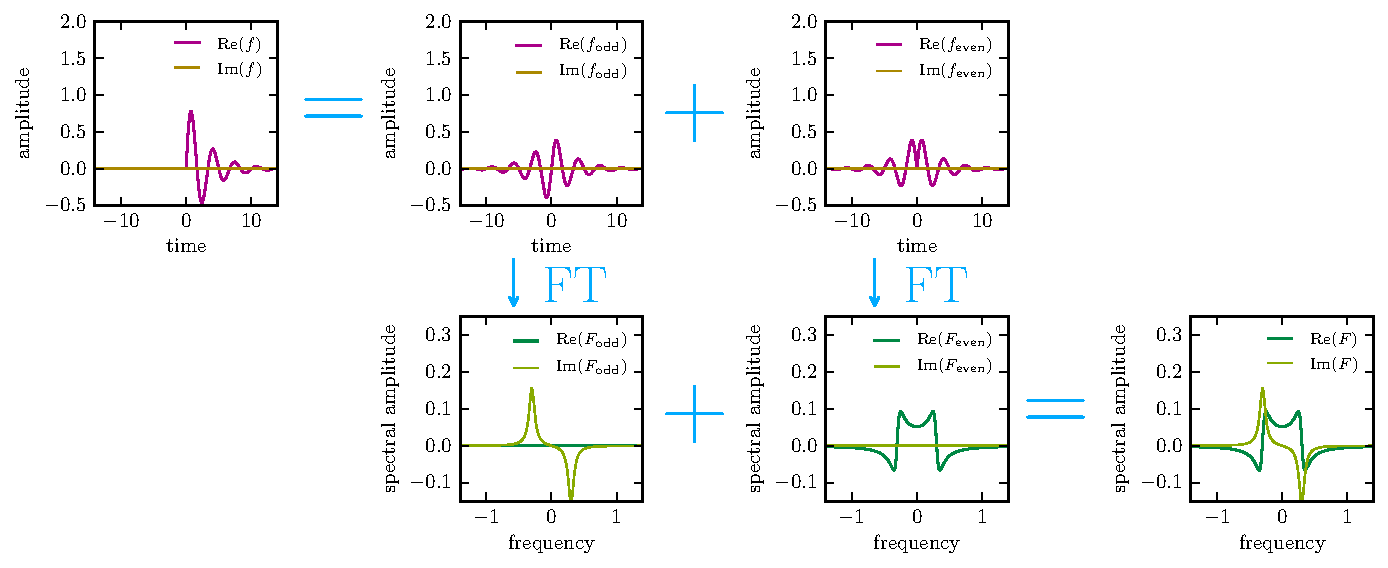
\includegraphics[width=17.5cm]{img/Kramers_Kronig_plot/kk.pdf}
\end{figure}
The Fourier transform of a real odd function is an imaginary function:
%F_{odd}(\omega)=& \int_{-\infty}^{\infty} e^{-\ii \omega t} f(t) \mbox{d}t = \\
		 %=&  \frac{1}{2} \int_{0}^{\infty} e^{-\ii \omega   t } [ f_{odd}(t) + f_{even}(t)] \mbox{d}t 
		   %+ \frac{1}{2} \int_{0}^{\infty} e^{-\ii \omega (-t)} [-f_{odd}(t) + f_{even}(t)] \mbox{d}t  \\
		 %=&  \int_{0}^{\infty} \frac{e^{-\ii \omega t}-e^{+\ii \omega t}}{2} f_{odd}(t) \mbox{d}t 
		   %+ \int_{0}^{\infty} \frac{e^{-\ii \omega t}-e^{+\ii \omega t}}{2} f_{odd}(t) \mbox{d}t  = \\
		 %=&\int_{-\infty}^{\infty} e^{-\ii \omega t} f(t) \mbox{d}t  = \\
		 %=&\int_{-\infty}^{\infty} e^{-\ii \omega t} f(t) \mbox{d}t  = \\
\begin{equation} 
\begin{split} 
F_{odd}(\omega)=& \int_{-\infty}^{+\infty} e^{-\ii \omega t} f_{odd}(t) \,\mbox{d}t = 
		 \int_{-\infty}^{+\infty} \frac{e^{-\ii \omega   t }}{2} f_{odd}(t) \,\mbox{d}t 
		   +  \int_{-\infty}^{+\infty} \frac{e^{-\ii \omega (-t)}}{2} [-f_{odd}(-t)] \,\mbox{d}t  \\
		 =&   \int_{-\infty}^{+\infty} \frac{e^{-\ii \omega t}-e^{+\ii \omega t}}{2} f_{odd}(t) \,\mbox{d}t 
		 = -\ii \underbrace{\int_{-\infty}^{+\infty} \sin(\omega t) \, f_{odd}(t) \,\mbox{d}t}_{\mbox{$\in \mathbb{R}$}},
\end{split} 
\label{eq_kkF}\end{equation}
whereas the Fourier transform of a real even function yields a real function:
\begin{equation} 
\begin{split} 
F_{even}(\omega)= \ldots =   \int_{-\infty}^{+\infty} \frac{e^{-\ii \omega t}+e^{+\ii \omega t}}{2} f_{even}(t) \,\mbox{d}t 
		 = \underbrace{\int_{-\infty}^{+\infty} \cos(\omega t) \, f_{even}(t) \,\mbox{d}t}_{\mbox{$\in \mathbb{R}$}}.
\end{split} 
%% TODO the following is WRONG! see ---->  http://www.thefouriertransform.com/pairs/step.php#signum,  ho3.pdf
\label{eq_kkFeven}\end{equation}
The odd and even components of the time-domain response function correspond to the imaginary and real part of the response spectrum, respectively:
\begin{equation} F_{odd}(\omega) + F_{even}(\omega) = F(\omega), \text{ where } F_{odd}(\omega) = F''(\omega) \text{ and } F_{even}(\omega) = F'(\omega).  \label{eq_kkFodd}\end{equation}
At the same time, $f_{even}(t)$ and $f_{odd}(t)$ are related to each other by having the opposite sign for $t<0$ and the same sign for $t>0$, that is 
\begin{equation} f_{even}(t) = \mbox{sign}(t)\,f_{odd}(t). \label{eq_kkfeven}\end{equation}
Multiplication in the time domain manifests as a convolution in frequency domain
\begin{equation} 
F_{even}(\omega) = \int_{-\infty}^{+\infty}  \frac{-2\ii}{\omega - \Omega} F_{odd}(\omega) \,\mbox{d}\Omega  \equiv  \left[\frac{-2\ii}{\omega}\right]\,\ast\,F_{odd}(\omega),
\label{eq_kkresult}\end{equation} 
where we used the knowledge that the $-2\ii/\omega$ function is the Fourier transform of $\mbox{sign}(t)$. Convolution with this function is also known as the Hilbert transform.% tODO cite

Obviously, Eq. (\ref{eq_kkfeven}) can also be converted to $f_{odd}(t) = \mbox{sign}(t)\,f_{even}(t)$, thus the relation between the real and imaginary part of the response spectrum also holds when $F_{odd}(\omega)$ and $F_{odd}(\omega)$ are exchanged in Eq. (\ref{eq_kkresult}). 

A related mathematical proof of Kramers-Kronig relations can be derived from the analyticity of the response function in the complex plane of frequency. %% TODO cite

%% TODO: why do K-K relations forbid to choose arbitrary phase difference over an unit cell? 
%% ie. Why the Neff can be unambiguously extracted from spectra?
% TODO show how it dictates the "constant area of imaginary part " when resonance Q is changed
%}}}

\subsection{Dispersion relations in local Drude-Lorentz media} \label{disp_rel_local_media}
\paragraph{Lower and upper polariton branches of transverse waves}  % TODO%{{{
Returning to the derivation of dispersion relations, we start with modifying the constitutive relation (\ref{eq_ce}) to a plane wave propagating in a medium:
\begin{equation}		\D := \varepsilon_0\epsrl(\omega)	\E, \quad\quad\quad						\B := \mu_0\mu_r(\omega)		\HH,				 \label{eq_ce2}\end{equation}
with the relative permittivity $\epsrl(\omega)$ and permeability $\mu_r(\omega)$ being two dimensionless functions of frequency, defined in Eq. (\ref{eq_lorentz_eps}, \ref{eq_lorentz_mu}). 
The wave equation (\ref{eq_wavek}) then changes to
\begin{equation}  T\E = \varepsilon_0 \mu_0  \epsrl(\omega) \murl(\omega) \, \frac{ \omega^{2}}{k^2} \E.  \label{eq_wavek_disp}\end{equation}
For transverse waves in isotropic media, the electric field is perpendicular to the wave vector ($T\E = \E$), and Eq. \ref{eq_wavek_disp} can be simplified to  
\begin{equation} k(\omega) = \sqrt{\varepsilon_0 \mu_0} \sqrt{\epsrl(\omega) \mu_{r}(\omega)}\;\omega = \sqrt{\epsrl(\omega) \mu_{r}(\omega)}\; \frac{\omega}{c}, \label{eq_dispeq_loc}\end{equation}
with the added frequency-dispersive term responsible for the deviation of Fig. \ref{fg_dcsimpleel} from the original straight light line in Fig. \ref{fg_dcvac}. 





In the simplest example of a single electric resonance with negligible losses, as in Fig. \ref{fg_dcsimpleel}, the curve is divided into two separate branches. The \textit{lower polariton branch} is below the resonance frequency $\omega_0$ and is characterized by the Lorentz oscillator being in phase with the electric field. Above $\omega_0$, the dipoles of the Lorentz oscillator can no more follow the electric field and are opposite to it, thus the response of the medium is negative. With further increase of the frequency, the permittivity crosses zero at the frequency $\omega_{\text{L}}$. %, > \omega_0 which allows the transverse wave to propagate. 
where the \textit{upper polariton branch} starts. In case of a Lorentz oscillator unaffected by the presence of others, the difference $\omega_{\text{L}} - \omega_0$ can be computed from the magnitude of the oscillator (using the Lydanne-Sachs-Teller relation) \cite{klingshirn2007semiconductor}.

The same behaviour is observed for a single resonance in the permeability $\mu_r(\omega)$, and will be typical also for the spectra of resonances of macroscopic structures described later.

Note that the formation of upper and lower polariton branches can be reinterpreted\cite{landau1984electrodynamics} using the theory of coupled oscillators as the result of \textit{anticrossing} between the oscillator at the frequency $\omega_0$ (forming a horizontal line) and the photon branch (forming a straight growing light-line).

When losses are present, the lower and upper polariton branches are connected by a smooth line of \textit{anomalous} dispersion and very high losses.  % TODO \ref{fg_dispersion_polariton}
%}}}
\paragraph{Longitudinal waves in dispersive media} %{{{
The wave equation in local dispersive media (\ref{eq_wavek_disp}) 
%\begin{equation} - \kk (\kk \cdot \E) + k^2 \E = \varepsilon_0 \epsrl(\omega) \mu_0 \murl(\omega) \omega^{2} \E, \tag{\ref{eq_wavek_disp} \again} \end{equation}
also allows the existence of longitudinal waves with electric field parallel to the wave vector $\E || \kk$. It was shown earlier that there is no solution for longitudinal waves in vacuum except for a static homogeneous field.

\begin{figure}[t] \caption{Influence of a single resonance in the real part of relative permittivity $\epsrl'(\omega)$ (magenta curve in the left panel) to the shape of dispersion curves in the right panel (green curve, computed using Eq. (\ref{eq_dispeq_loc}). The lower and upper polariton branches are separated by a spectral region $\omega \in (0.3, 0.65)$, where the wave does not propagate on an appreciable distance (nonzero losses yield a finite solution here, though).} \label{fg_dcsimpleel} \centering  %% TODO refto
	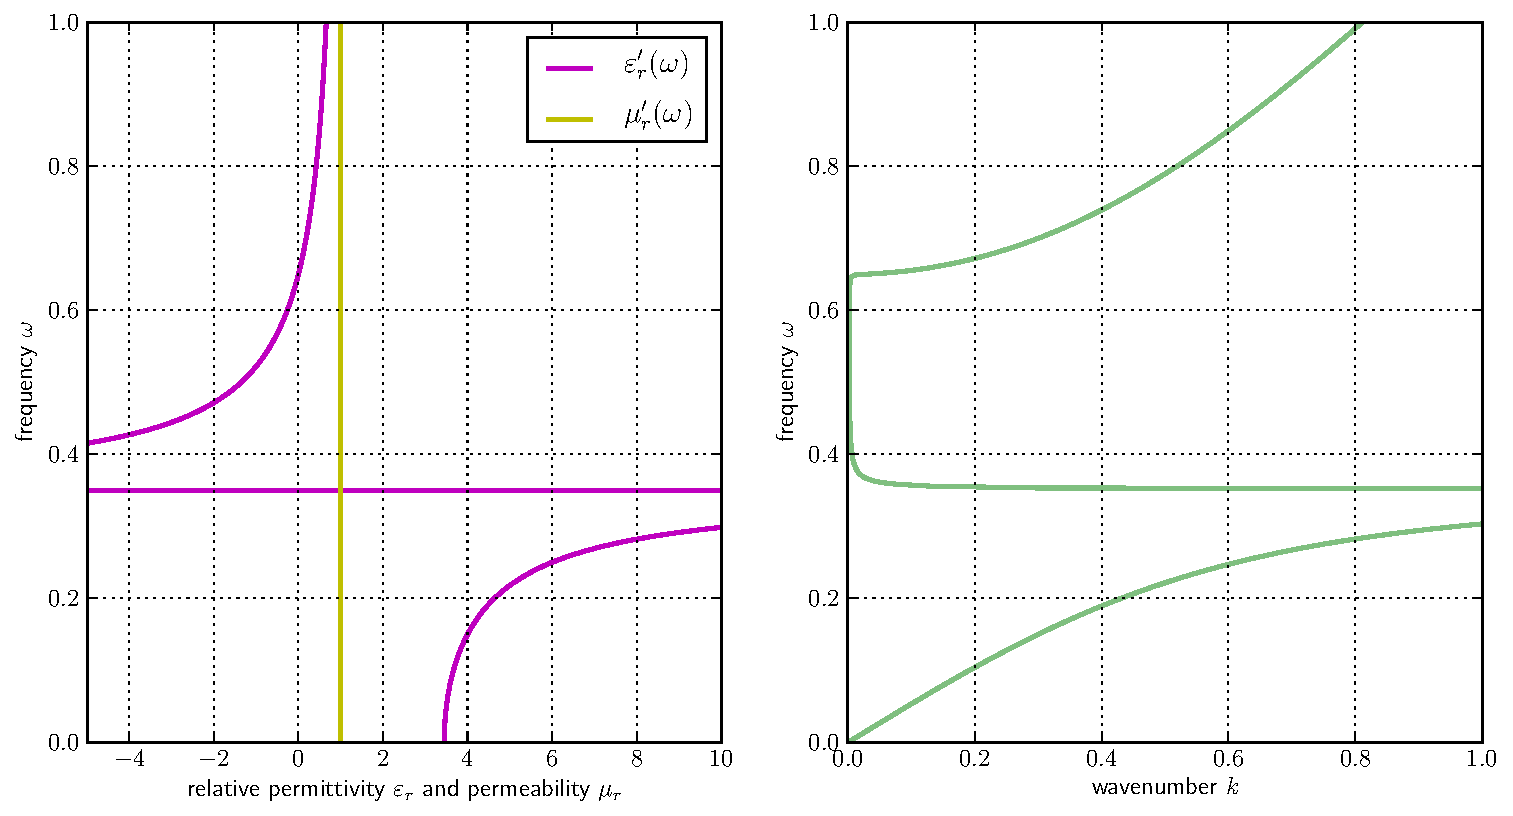
\includegraphics[width=17cm]{img/dispersion_landau_lifshitz/dispersion_simple_el.pdf}
\end{figure}
If a local medium is assumed, and the wavenumber $k$ is nonzero, such waves can have a solution with nonzero $\E$ when $\epsrl(\omega)' = 0$, or with nonzero $\HH$ when $\mu_r(\omega)' = 0$. Therefore, the corresponding dispersion curve for a longitudinal wave is a horizontal line at $\omega = \omega_{\text{L}}$, independent of $k$. This would be equivalent to a standing oscillation that maintains the spatial amplitude envelope that was originally excited. 

Different physical phenomena can lead to $\epsrl(\omega)' = 0$, some of which introduce relatively low losses at the corresponding $\omega_{\text{L}}$; namely lattice vibrations in nonconductive crystals or electrons in inductive media (like metals and dilute plasma). 

At the interface of two media with differing signs of permittivity, another type of waves can be excited with an intermediate frequency $\omega < \omega_{\text{L}}$ that can not propagate in either of the bulk medium. The dispersion curve of such waves is not flat, allowing them to propagate along the interface. Depending on the mechanism, they are known as  \textit{surface plasmons} or \textit{surface phonon-polaritons} \cite[p. 87]{klingshirn2007semiconductor}, respectively. Accordingly, \textit{surface magnons} should be observed at interfaces where $\mu$ changes its sign.
% Are there surface magnons?
% Are there any metamaterials designed for longitudinal waves?
%}}}
\paragraph{Anisotropy of permittivity} \label{par_anisotropy} %{{{
It shall be noted here that permittivity $\epsrl$ was introduced as a scalar, assuming that the vector of electric field $\E$ and electric induction $\D$ are always of the same orientation:
\begin{equation} \D = \varepsilon_0 \epsrl(\omega) \E \equiv \varepsilon_0  
	\left(\begin{array}{ccc} 
			\epsrl(\omega) & 0 & 0  \\
			0 & \epsrl(\omega) & 0  \\
			0 & 0 &\epsrl(\omega)  
	\end{array} \right) \cdot \E
	\label{eq_ed_orientation}
\end{equation}
In some media of lower rotational symmetry (such as many crystals, or liquids under static electric field), the medium response depends on the electric field direction. At the beginning of the chapter, however, we assumed the fields are relatively weak, and we imposed the requirement of \textit{linearity} of the medium. Whatever the linear relation of $\D := \mathcal{L}(\E)$
is, it must obey the rule
$$\D_1 + \D_2 = \mathcal{L}(\E_1) + \mathcal{L}(\E_2) = \mathcal{L}(\E_1 + \E_2)$$
for any vectors $\E_1, \E_2$. Such a relation can be fully described by a \textit{tensor of permittivity} % TODO cite 
\begin{equation} \D = \varepsilon_0 \epsrl(\omega) \E \equiv \varepsilon_0  
	\left(\begin{array}{ccc} 
	{\epsrl}_{xx}(\omega) & {\epsrl}_{xy}(\omega) & {\epsrl}_{xz}(\omega)  \\
	{\epsrl}_{yx}(\omega) & {\epsrl}_{yy}(\omega) & {\epsrl}_{yz}(\omega)  \\
	{\epsrl}_{zx}(\omega) & {\epsrl}_{zy}(\omega) & {\epsrl}_{zz}(\omega)  
	\end{array} \right) \cdot \E.
	\label{eq_epstensor}
\end{equation}
Elaborate discussion on all possible forms of this tensor and their physical interpretation can be found e.g. in \cite[pp. 678--686]{born1999book}. An analogous treatment can be applied to the magnetic permeability, though it is less often needed.

%}}}
\paragraph{Dispersion relations in anisotropic local media}  %{{{
If the medium response depends on the direction of the field, the dispersion relations can not be directly obtained by substitution into the wave equation as in Eq. % \ref{}. 

%\begin{equation} xxx  T\E :=  -\frac{\kk (\kk \cdot \E)}{k^2} + \E            = \frac{\mu_0 \varepsilon_0 \omega^{2}}{k^2} \E.  \label{eq_wavek}\end{equation}
%\begin{equation} xxx - \kk (\kk \cdot \E) + k^2 \E = \varepsilon_0 \epsrl(\omega) \mu_0 \murl(\omega) \omega^{2} \E,  \end{equation}

%is a linear transformation of the vector $\E$, which can be expressed by the tensor
%$$ - \kk (\kk \cdot \E) \equiv 
	%-\left(\begin{array}{c} k_x \\ k_y \\ k_z \end{array} \right) \cdot
	%\left[\left(\begin{array}{ccc} k_x & k_y & k_z \end{array} \right) \cdot
	%\left(\begin{array}{c} E_x \\ E_y \\ E_z \end{array} \right)\right] 
		%\equiv
	%\left(\begin{array}{ccc} -k_x^2 & -k_x k_y & -k_x k_z \\ -k_y k_x & -k_y^2 & -k_y k_z \\ -k_z k_x & -k_z k_y & -k_z^2 \end{array} \right) \cdot  
	%\left(\begin{array}{c} E_x \\ E_y \\ E_z \end{array} \right).
	%$$
%$$ k^2 \E \equiv 
%	\left[\left(\begin{array}{ccc} k_x & k_y & k_z \end{array} \right) \cdot 
%	\left(\begin{array}{c} k_x \\ k_y \\ k_z \end{array} \right)\right] \cdot 
%	\left(\begin{array}{c} E_x \\ E_y \\ E_z \end{array} \right),
%	$$
%$$ \mu_0 \varepsilon_0 \omega^{2} \E \equiv 
%	\left(\begin{array}{ccc} k_x^2+k_y^2+k_z^2 & 0 & 0 \\ 0 & k_x^2+k_y^2+k_z^2 & 0 \\ 0 & 0 & k_x^2+k_y^2+k_z^2 \end{array} \right) \cdot  
%	\left(\begin{array}{c} E_x \\ E_y \\ E_z \end{array} \right),
%	$$
The dispersion relation can however still be understood \cite[pp. 667]{born1999book} as a set of three linear algebraic equations:
\begin{equation}  T\E =  -\frac{\kk (\kk \cdot \E)}{k^2} + \E            = \frac{\varepsilon_0 \mu_0 \, \epsrl(\omega) \murl(\omega) \omega^{2}}{k^2} \E. \tag{\ref{eq_wavek_disp} \again}\end{equation}
%\begin{equation} \left|\begin{array}{ccc} 
	%k_y^2+k_z^2 - \mu_0 \varepsilon_0 \omega^{2} 		& -k_x k_y 		& -k_x k_z \\ 
	%-k_y k_x 		& k_x^2+k_z^2-\mu_0\varepsilon_0\omega^{2} 		& -k_y k_z \\ 
	%-k_z k_x 		& -k_z k_y		& k_x^2+k_y^2-\mu_0\varepsilon_0\omega^{2}
	%\end{array} \right| = 0, \label{eq_dispdet}\end{equation}
where the wave-plane projection tensor $T$, dependent on the wavevector $\kk$, was already defined in Eq. (\ref{eq_transverse1}).

For simplicity, we assume here that the relative permeability $\murl = 1$; the extension to other cases is possible, too. %% TODO Do epsilon and mu commute, if they are both tensors??
A solution of Eq. \ref{eq_wavek} can exist with nonzero $\E$ if and only if the determinant of the set of three linear equations is zero:
\begin{equation} 
\det\left[
T -
	\frac{\mu_0 \varepsilon_0 \omega^2}{k^2}
	\left(\begin{array}{ccc} 
	{\epsrl}_{11}(\omega) & {\epsrl}_{21}(\omega) & {\epsrl}_{31}(\omega)  \\
	{\epsrl}_{12}(\omega) & {\epsrl}_{22}(\omega) & {\epsrl}_{32}(\omega)  \\
	{\epsrl}_{13}(\omega) & {\epsrl}_{23}(\omega) & {\epsrl}_{33}(\omega)  
	\end{array} \right) \right] = 0, \label{eq_dispdet}\end{equation}
The search for dispersion curves in an anisotropic medium is thus transformed into finding zeroes of this function of four scalar variables, $k_x$, $k_y$, $k_z$ and $\omega$.
In the most general case, it can be solved by means of numerical algebra software. 

\todo{add about the number of solutions}
%For a given frequency $\omega$, rigorous solution of Eq. \ref{eq_dispdet} in local media gives in fact three solutions, of which two are for different polarisations of a transverse wave, and the third is for the longitudinal wave. The two transverse solutions give identical wave vector (are degenerate) if the medium is isotropic, or if $\kk$ points along the optical axis. 
% The longitudinal wave ... ?

%}}}
\paragraph{Isofrequency contours}  %{{{
%A resonance in local permittivity (or permeability) creates two polariton branches -- thus the dispersion curves can not be expressed as one simple function $\omega(k)$ of the wavevector $k$. It would then appear adequate to treat dispersion curves as a function of frequency, $k(\omega)$, but as is shown below in the presence of nonlocal response, neither $k$ is necessarily a simple function of $\omega$. Also 
It is often important to describe the dispersion curves also for different wave angles, which is the best accomplished by plotting the  %% todo ...real part of ...
frequency $\omega$ as the function of \textit{wave vector} $\kk$. In three dimensions, this would require mapping a function of three independent variables, $\omega(\kk) = \omega(k_x, k_y, k_z)$. However, in most cases the projection of two selected components of $\kk$ is sufficient to understand all relevant phenomena, and naturally it is much easier to visualize. 
\begin{figure}
  \begin{minipage}[c]{0.5\textwidth}
\hfill
    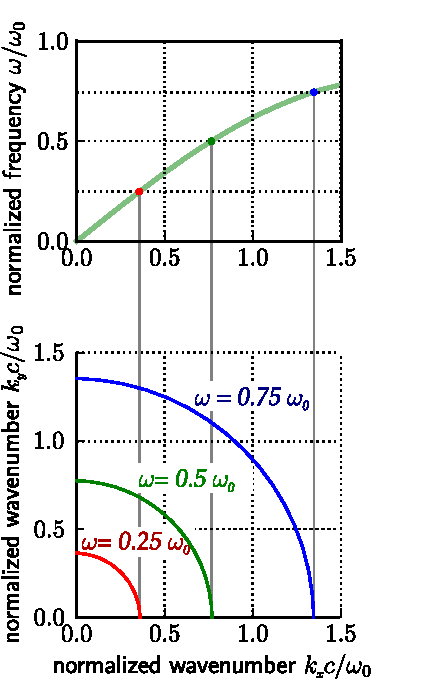
\includegraphics[width=7cm]{img/dispersion_curves_to_ifc.pdf}
  \end{minipage}
  \begin{minipage}[c]{0.5\textwidth}
    \caption{The relation between a plot of a dispersion curve for one photonic branch and the corresponding isofrequency contours. At a selected frequency, all points in the $k_x$-$k_y$ plane are drawn for which a nonzero solution of Maxwell equations exists. For transverse waves in local media, this is equivalent to finding a solution to the dispersion equation (\ref{eq_dispeq_loc}).\\Multiple frequencies can be plotted to describe the frequency dependence. For illustration, an isotropic medium was used, thus all IFCs take the form of a circle. To save space, only one quarter of the circle was plotted here.} \label{fg_ifc_dc}
  \end{minipage}
\end{figure}

Such a plot is known as \textit{isofrequency contours} (IFC), or also \textit{equifrequency contours} (EFC), and allows for intuitive geometrical analysis of various phenomena such as light refraction, beam walk-off, total internal reflection etc. 
The relation between a dispersion curve for one photonic branch and the corresponding isofrequency contours in an isotropic medium is shown in Fig. \ref{fg_ifc_dc}.

Its limitation is, however, that IFC plots do not show the imaginary part and thus are applicable to plot the dispersion in media with no or negligible losses only.  
Each photonic branch also has to be plotted in a separate plot to prevent the contours from overlapping (see the right panel of Fig. \ref{fg_dcsimpleel}). 
Moreover, in every single photonic branch, Eq. \ref{eq_dispdet} yields two solutions for two possible polarisations of transverse waves \cite[p. 46]{klingshirn2007semiconductor}. The IFCs for these solutions are generally different in anisotropic media, but we always restrict the discussion only one polarisation in the following figures  for simplicity. % \todo{discuss? In uniaxial media, where two diagonal components of the }

\begin{figure}[ht] \caption{\textbf{(a)} Isofrequency contours for an isotropic medium are circular and centered in the $k=0$ point.  
		\textbf{(b)} An anisotropic medium with the optical axis perpendicular to the interface, where IFCs take the form of ellipses. \textbf{(c)} A similar case of another anisotropic medium, with the orientation of the optical axis (drawn as the dashed black line) that enables to introduce the index of refraction for the shown direction of the wave vector $\kk$.
%% FIXME \textbf{(d)} A dispersive \textit{hyperbolic medium}, with one component being a function of frequency and crossing zero.
} \label{fg_ifc} \centering  %% TODO verify in Belov that local media may be used  as hyperbolic
	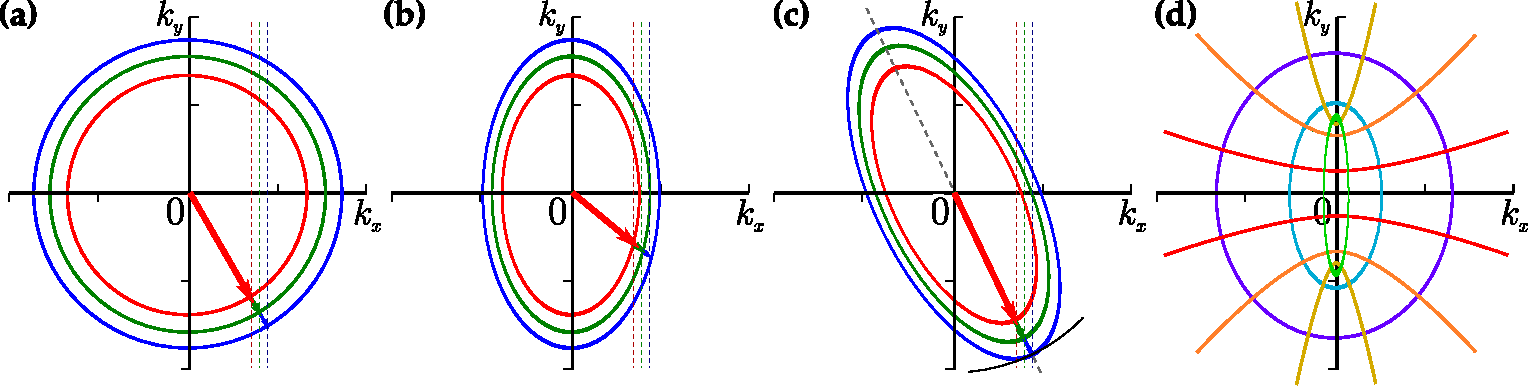
\includegraphics[width=.8\textwidth]{img/ifc_freqdispersion.pdf} 
\end{figure}
Isofrequency contours are valuable for graphical prediction of wave refraction on interface of two media \cite[p. 118]{shalaev2010book}. Starting, e.g., in the isotropic medium in Fig. \ref{fg_ifc}a, the wavevectors are known for given frequencies (as three coloured arrows).
The component of wave vector parallel to the interface (chosen as $k_x$ here and indicated by the vertical dashed lines) must be maintained upon refraction. This rule can be intuitively deduced from the continuity of the wave phase at the interface, as well as from the Noether theorem applied to the infinite translational symmetry of the interface. Transferring the vertical dashed lines to IFC plot of another medium and finding the intersections with an IFC of the corresponding frequency, one can find the new wavevector. 
In Fig. \ref{fg_ifc}, we provide examples of IFCs for one isotropic and two anisotropic media.

%}}}
\paragraph{Index of refraction and its applicability}  %{{{
With the background of the theory developed above, the notion of the \textit{index of refraction} $N$ can be properly introduced and discussed. 
In the most strict sense, the index of refraction is defined only for \textit{isotropic} media. Then it is equivalent to the ratio of the wavenumber $k(\omega) \equiv |\kk|$ to the wavenumber in vacuum at the same frequency: 
\begin{equation} N(\omega) := k(\omega) \, \frac{c}{\omega} \equiv \sqrt{\epsrl(\omega)\murl(\omega)}, \label{eq_dispeqN}\end{equation}
as directly follows from Eq. (\ref{eq_dispeq_loc}).

Starting with a harmonic plane wave with the frequency $\omega$ and the wave vector $\kk^{(1)}$ refracting at an interface of two isotropic media, the projection of $\kk$ to the interface is given as 
$$ k_x = k^{(1)}\,\sin \alpha^{(1)}, $$
where $\alpha^{(1)}$ is the angle between the wavevector in the first medium $\kk^{(1)}$ and the  normal to the interface. In the second medium, a similar relation must apply, however the wavenumber $k^{(2)}$ may be different and as a result, the angle in the second medium is
\begin{equation} \alpha^{(2)} = \arcsin\left( \frac{k^{(1)}}{k^{(2)}} \,\sin \alpha^{(1)} \right) = \arcsin\left( \frac{N_1}{N_2} \,\sin \alpha^{(1)} \right), \label{eq_snell}\end{equation}
which is known as the \textit{Snell} (or also \textit{Snell-Descartes}) law.

The majority of (effective) media discussed in this thesis are however more or less anisotropic, and somewhat surprisingly, the notion of \textit{index of refraction} $N$ seems to be widely used for them in the literature anyway. The author thus feels there is a need for a conscientious extension of $N$ for anisotropic cases, too. An extremely loose definition of $N$ could be based on computing the ratio $N(\omega, \kk) := kc/\omega$  for any medium. This can be formally done, but then the wavenumber $k$ would also depend on the direction $\alpha$, and the Snell law in Eq. (\ref{eq_snell}) would become an implicit equation, losing its original purpose of making the computation explicit and notably simple.

The author proposes instead to restrict the term \textit{index of refraction} to all cases where IFCs are perpendicular to $\kk$. This covers not only all isotropic media, but also those cases when the waves propagate close the optical axis of any anisotropic media. An example of an anisotropic medium with its optical axis oriented in such a way that the refraction can be computed using Snell law provided the $k_x$ component is shared with \ref{fg_ifc}a, is shown in Fig. \ref{fg_ifc}c. For small deviations from this angle, where the IFC can be approximated by an osculating circle, 
\begin{equation} \frac{\partial k}{\partial \alpha} \ll k,\label{eq_osculating}\end{equation}
the Snell law still gives a correct prediction of the refraction angle. 

We will however show in the following that the prediction of \textit{beam} propagation is more complicated, being sensitive to the \textit{curvature of IFC}. 

%}}}
%%   \paragraph{Isofrequency contours of hyperbolic media}  %{{{ TODO READ BELOV2003 and FIXME
%%   The IFCs in Fig. \ref{fg_ifc}a,b,c were plotted for non-dispersive media, i. e. with $\epsrl$ and $\murl$ independent of frequency. The case of one polariton branch of a dispersive isotropic medium is already shown in Fig. \ref{fg_ifc_dc}, characteristic by non-equidistant IFCs which lead to the refraction angle being dependent on the frequency.
%%   
%%   A more complicated cases are the \textit{hyperbolic media}, where, in a certain spectral region, one component of the anisotropic permittivity is positive, while another one is negative. The solution of Eq. (\ref{eq_dispdet}) then results in a hyperboloid, which is either of one sheet or two sheets, depending on the sign of the remaining diagonal component of permittivity tensor. At the frequencies where the dispersive component of permittivity is negative,  
%%   Note that a negative permittivity is always connected with the dispersive behaviour, thus \ref{fg_ifc}d is another example of a dispersive medium. 
%%   
%%   %}}}
\paragraph{Group velocity}  %{{{  todo near single resonance
So far only the propagation and refraction of an infinite, single-frequency wave was discussed, and it was shown that it is determined by the shape of IFC at the given frequency. %% todo rewrite to more precise

If the wave is temporally modulated, its envelope in time is given as a complex vector function $\E_0(t)$ replacing the constant vector $\E_0$ in Eq. \ref{eq_pw}. This can be equivalently expressed in the frequency domain as the wave being formed by superposition of multiple frequency components, with respective amplitudes given by the Fourier transform of $\E_0(t)$. The position of the envelope in time is determined by their \textit{mutual phase difference}, not by the absolute wave phase. 

A similar argument can be made regarding the spatial modulation of the wave. Any wave shape other than the infinite plane wave is a superposition of waves with different wavevectors, and the direction of propagation of the spatial envelope is given by mutual phase difference of the constituent waves. % TODO rewrite-unclear

The velocity vector of the envelope propagation, denoted as the \textit{group velocity} $\mathbf{v_g}$, can be found as the gradient of frequency by the wavevector: %% TODO cite
\begin{equation} \mathbf{v_g} := \frac{\partial \omega}{\partial \kk} \equiv 
\left(\begin{array}{c} 
	\partial \omega/\partial k_x \\ 
	\partial \omega/\partial k_y \\ 
	\partial \omega/\partial k_z \\ 
	\end{array} \right)
 \label{eq_vg}\end{equation}
In the IFC plot, the group velocity can be visually found as directing always perpendicular to the IFC, with its magnitude being proportional to the density of the IFCs.

If the group velocity is different from the phase velocity, the envelope $\E_0(t)$ is maintained over time, but it continuously shifts against the underlying wave. Thus the actual temporal shape of $\E(t)$ changes upon passing through a dispersive medium.
On the contrary, in vacuum or media with negligible dispersion, each frequency component of the wave acquires an additional phase strictly proportional to its frequency. Then the group velocity coincides with the phase velocity: 
$$\hspace{3cm}\mathbf{v_g} = \kk \omega / k^2 \hspace{3cm} \text{(in nondispersive isotropic media)}.$$
%The orientation of $\vg$ and $\kk$ is usually the same, but later it will be shown that it can be otherwise, with peculiar physical consequences.

Usually in spectral regions near a resonance, also the quadratic or even higher terms in the Taylor expansion of the $\omega(\kk)$ dependence shall be taken into account. This effect is known as the \textit{group velocity dispersion} as it is equivalent to the group velocity $\vg(\kk)$ being dependent on the wavevector (or, if reformulated, on frequency). It results in temporal distortion of the wave envelope $\E_0(t)$.  %% TODO ... and what about distortion in space?
%}}}
\paragraph{Propagation of a beam in anisotropic media}  %{{{  
The refraction of a beam is illustrated in Fig. \ref{fg_ifc2} by means of three slightly different wavevectors it is composed of. For simplicity, a monochromatic wave was used, so brown, black and violet were chosen for the three example wavevectors to prevent confusion with the rainbow-like frequency color map used in Fig. \ref{fg_ifc}. 

In the first plot, \ref{fg_ifc2}a, the case of an isotropic medium is illustrated. Upon refraction into a general anisotropic medium in Fig. \ref{fg_ifc2}b, each component must maintain its wavevector projection to the interface, thus the wavevectors spread in their direction. The resulting beam propagates along the group velocity that is different from the central wavevector; % The components of the resulting beam are   is narrower and does not propagate 
this is also known as the spatial \textit{walk-off}.
\begin{figure}[ht] \caption{Examples of IFCs similar to Fig. \ref{fg_ifc}, but now at a single frequency and different wavevectors, corresponding to a monochromatic beam refracting on the interface. \textbf{(a)} The wavevectors in the isotropic medium lie on a circle.
		\textbf{(b)} Generally, anisotropic media exhibit different orientations of the wave vector $\kk$ and the beam propagation. \textbf{(c)} For the special cases of propagation along the optical axis, the beam refracts similarly as in isotropic media.
 \textbf{(d)} In anisotropic media with hyperbolic shape of the IFC, the beam refracts to the opposite direction than the wave vector. } \label{fg_ifc2} \centering 
	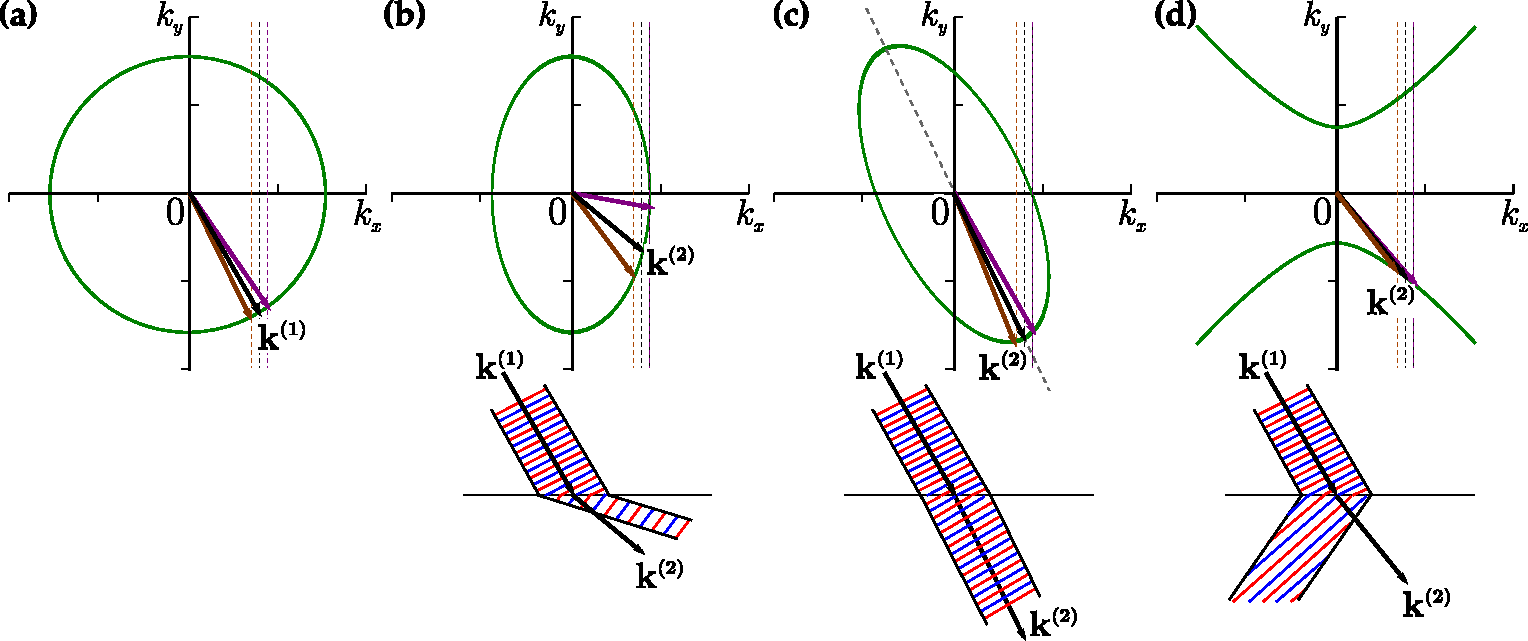
\includegraphics[width=\textwidth]{img/ifc_kdispersion_hyp.pdf} 
\end{figure}

Fig. \ref{fg_ifc2}c shows again the special case of the anisotropic medium, where the wave propagates near an optical axis, and thus where the Snell law can still be used to determine the refraction of a plane wave, based the generalized notion of the index of refraction.
However, there is a pitfall if one tries to apply the Snell law for prediction of how the beam will refract. The problem originates from the differential nature of the group velocity definition in Eq. (\ref{eq_vg}). 
%While the magnitude of the wavevector changes only negligibly, with the square of a 
While the phase velocity of a monochromatic wave at the frequency $\omega_0$ does not appreciably change upon a small deviation of the angle $\alpha$ from the optical axis  [c.f.  Eq. (\ref{eq_osculating})], the group velocity direction does, because it has a nonzero linear component in its dependence on the wavevector:
$$ \frac{\partial \vg(\kk)}{\partial \alpha} \neq 0.$$
As a result, the group velocity in anisotropic media is always much more sensitive to the angle than the phase velocity, and Snell law does not predict it correctly. It can be regarded as a spatially-dependent manifestation of the group velocity dispersion.

In Fig. \ref{fg_ifc2}d, an extreme case of spatial walk-off is shown on the example of a \textit{hyperbolic} medium with different signs of the permittivity along different axes. %% TODO study Belov2003 and possibly correct this if hyperbolas are wrong
 The normal to its IFC is nearly perpendicular to the wavevector, and accordingly, the beam refracts in opposite angle with regards to the incident wave. The $k_x$ component of the wave vector is however still maintained. A further geometrical development of the beam refraction is in Ref. \cite[p. 46]{klingshirn2007semiconductor}.

%If the amplitude and phase of the wave is not  temporal shape of a wave can be composed as a superposition of different frequency components with certain amplitude and phase. Similarly, any spatial shape of a beam can be composed of infinite waves of different wavevectors. The isofrequency contours, and their dependence on frequency, allow to determine how the temporal and spatial envelope will propagate. 
%Assuming a short pulse for simplicity

%}}}
\paragraph{The sign of the phase and group velocities}  %{{{
In the discussion of refraction both in Fig. \ref{fg_ifc} and \ref{fg_ifc2}, the solution of the vertical wave vector component $k_y$ pointing downwards was always selected without providing justification. In fact, both upwards and downwards pointing wave vector provide valid solution. The reason is that in the first medium represented by the leftmost plots (Fig. \ref{fg_ifc}a and \ref{fg_ifc2}a), the incident wave was propagating downwards to the interface, and it was assumed that also the refracted wave will propagate downwards, from the interface.

A more complicated case occurs when the wave vector $\kk$ and group velocity $\vg$ point in opposite direction (or more generally, when they have an opposite projection on the normal to the interface).  This manifests as IFC radius \textit{decreasing} with frequency growing, as shown in  Fig. \ref{fg_ifcnr}.
Such a case can indeed occur in natural or artificial media, as described in more detail below. 
\begin{figure}[ht] \caption{Frequency-dependent IFCs of \textbf{(a)} an ordinary medium, \textbf{(b)} an isotropic medium with a negative index of refraction and \textbf{(c)} an anisotropic medium with a negative index of refraction \todo{comment}} \label{fg_ifcnr} \centering  %% TODO  WRITE
	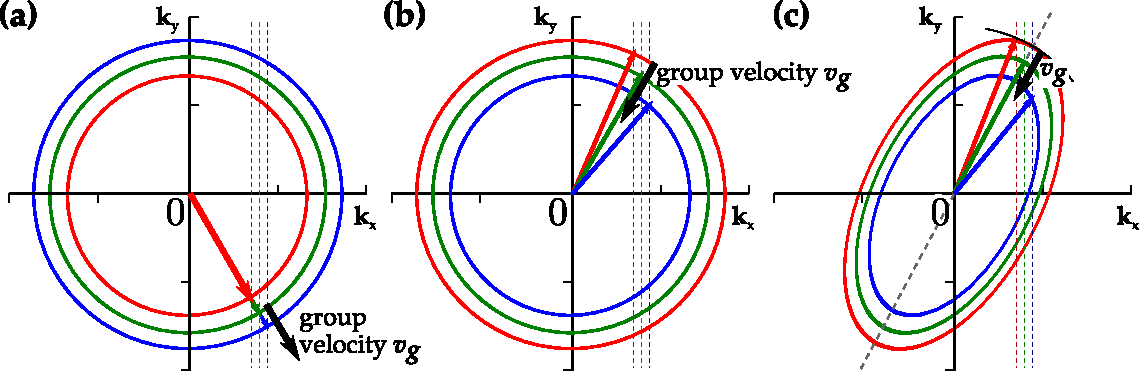
\includegraphics[width=.8\textwidth]{img/ifc_negrefr.pdf} 
\end{figure}
\begin{figure}[ht] \caption{Wavevector-dependent IFCs for one frequency, for media choice the same as in Fig. \ref{fg_ifcnr} \todo{extend}} \label{fg_ifcnrk} \centering  %% TODO  WRITE
	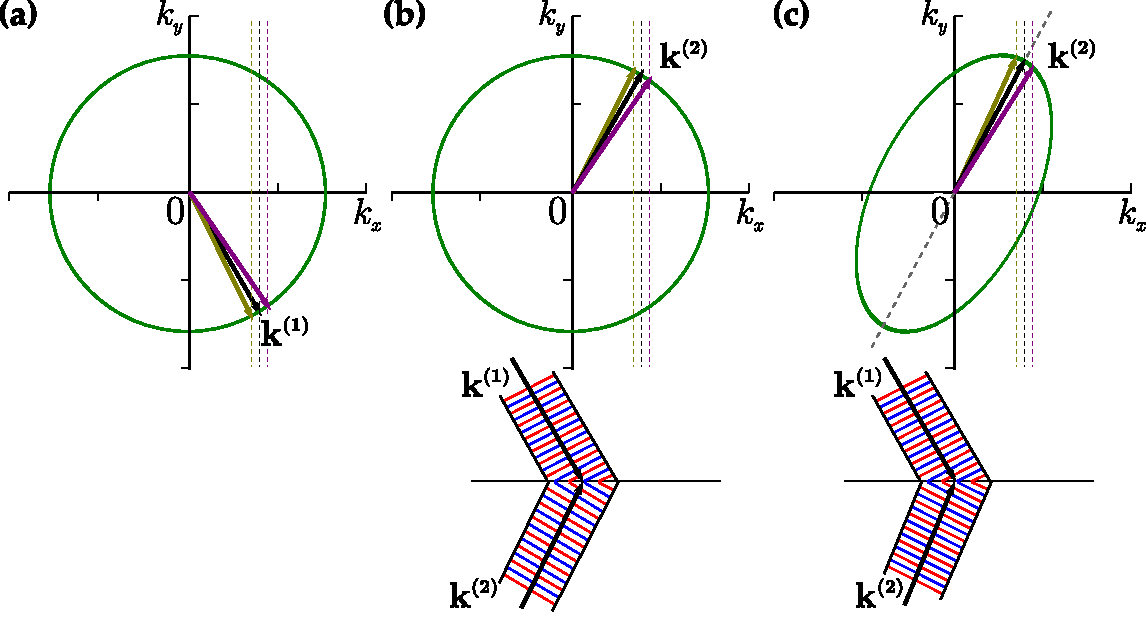
\includegraphics[width=.8\textwidth]{img/ifc_negrefrk.pdf} 
\end{figure}

In the isotropic media, or the media where the wave vector points in direction close to the optical axis, the Snell law is still applicable, and we then speak of \textit{negative index of refraction}.  The refraction between an ordinary medium and two examples of negative-index media are plotted in Fig. \ref{fg_ifcnr}.
It should be noted that the negative-index media are necessarily dispersive. Therefore, the refraction of temporally short pulses disperses different frequencies into different angles, as can be found from the wavevectors at different frequencies in Fig. \ref{fg_ifcnr}b,c.

\todo{add that the propagation velocities are more complicated than this and will be discussed later; move a part of this text below?}
%}}}

\subsection{Nonlocal response} 
\paragraph{Definition of nonlocal media}%{{{
%TODO: spatial dispersion describes one specific sort of nonlocal behaviour that exists in homogeneous infinite media only
The previous two chapters that concerned local media can be generalized into the theory of \textit{nonlocal} (or, \textit{spatially dispersive}) media that follows.

The downsides of the spatial-dispersive model of media is that it is more complicated, leading e.g. to an implicit dispersion equation. Its great advantage is however that it provides a necessary level of generality for the description of periodic structures discussed below. 
Some phenomena observed in the frequency spectrum are in fact consequences of the spatial dispersion, such as the Doppler broadening of resonance lines in gases \cite[p. 359]{landau1984electrodynamics}. More precisely, these phenomena are primarily dependent on the wave vector $\kk$, and their expression by means of the temporal spectrum is a mere approximation based on that the dispersion curve usually defines a simple relation between  frequency and wave vector.  %% TODO rewrite?

In this section such a more general class of media is discussed, where the medium response explicitly depends on the history of $\E(\tau, \brho)$ in previous time $\tau < t$ and in all surrounding points $\brho$, and therefore is described by a spatio-temporal convolution:
\begin{equation} \D(t,\rr) = \varepsilon_0 \E(t,\rr) + \varepsilon_0\int_{V} \int_{-\infty}^{t} \chi_e(t-\tau, \rr-\brho) \, \E(\tau,\brho) \,\mbox{d}\tau \,\mbox{d}^3\brho. \label{eq_chi_convol_nonloc}\end{equation}
In a very similar manner as in the local theory above, we assume a plane wave $\E(t, \rr) := \E_0 \, e^{\ii\omega t - \ii\kk\cdot\rr}$ propagates through the medium. This is without loss of generality, thanks to that it is possible to express any wave as a superposition of monochromatic plane waves.
\begin{equation} \D(t,\rr) = \varepsilon_0 \E_0 \, e^{\ii\omega t - \ii\kk\cdot\rr} + \varepsilon_0\int_{V} \int_{-\infty}^{t} \chi_e(t-\tau, \rr-\brho) \, \E_0 \, e^{\ii\omega \tau - \ii\kk\cdot\brho} \,\mbox{d}\tau \,\mbox{d}^3\brho. \label{eq_chi_convol_harm_nonloc}\end{equation}
After two  substitutions, $T:=t-\tau$, $\mathbf{R}:=\rr-\brho$, the exponent can again be separated into the original plane wave (which factors out), and a spatio-temporal Fourier transform of the medium response:
$$				 \D(t,\rr) = \varepsilon_0 \E_0 \, e^{\ii\omega t - \ii\kk\cdot\rr} + \varepsilon_0\int_{V} \int_{-\infty}^{0} \chi_e(T, \mathbf{R}) \, \E_0 \, e^{\ii\omega (t - T) - \ii\kk\cdot(\rr - \mathbf{R})} \,\mbox{d}T \,\mbox{d}^3\brho,$$
$$				 \D(t,\rr) = \varepsilon_0 \E_0 \, e^{\ii\omega t - \ii\kk\cdot\rr} + \varepsilon_0\left( \int_{V} \int_{-\infty}^{0} \chi_e(T, \mathbf{R})  \, e^{-\ii\omega T + \ii\kk\cdot \mathbf{R}}\,\mbox{d}T \,\mbox{d}^3 \mathbf{R} \right) \E_0 \, e^{\ii\omega t - \ii\kk\cdot\rr}.$$
The response of the medium to the electric field of any harmonic plane wave can now be expressed as a function of frequency $\omega$ and wave vector $\kk$. It is defined as the ratio between the electric displacement and the electric field:
\begin{equation} \epsrn(\omega, \kk) = \left.\frac{\D(t,\rr)}{\varepsilon_0 \E(t,\rr)} \right|_{\E(t, \rr) := \E_0 \, e^{\ii\omega t - \ii\kk\cdot\rr}}  = 1 + \int_{V} \int_{-\infty}^{0} \chi_e(T, \mathbf{R}) \,e^{-\ii\omega T + \ii\kk\cdot \mathbf{R}} \,\mbox{d}T \,\mbox{d}^3\mathbf{R} \label{eq_eps_nonloc}\end{equation}
Converting the problem from the spatio-temporal domain into the wavenumber-frequency domain allows to express the relation between $\D$ and $\E$ by the \textit{permittivity} function $\epsrn(\omega, \kk)$ and completely avoid the convolution from Eq. (\ref{eq_chi_convol_harm_nonloc}). Note that both the response function $\chi_e$ and the permittivity $\epsrn$ %% TODO make it \varepsilon_r
may be either scalar functions, or rank-2 tensor functions; the latter case accounts for possible anisotropy of the medium.
% , and convolution in space is equivalent to multiplication  in the reciprocal space

The terms of \textit{nonlocality} and of \textit{spatial dispersion} are used interchangeably in the literature. The difference seems to be related to the way one thinks about the medium -- while \textit{nonlocality} is obviously related to the description in the real space [cf. Eq. (\ref{eq_chi_convol_nonloc})], \textit{spatial dispersion} derives from that the response is not a constant function in the reciprocal $\kk$-space. In the author's view, the term \textit{spatial dispersion} is therefore of slightly narrower meaning, as it implies that a plane wave of a defined wavevector is considered in an infinite medium.

%}}}
\paragraph{Power expansion of the medium parameters} %{{{
Assuming the dependence of the medium permittivity $\epsrn(\omega,\kk)$ or permeability $\murn(\omega,\kk)$ is a function varying slowly with $\kk$, we can express them in general as power series \cite[p. 367]{landau1984electrodynamics}:
\begin{equation} 
\left.  \begin{array}{c}
\epsrn(\omega,\kk) = 1 + \chi_e(\omega) + \ii \gamma_{\text{e}}(\omega) \kk + [\alpha_{\text{e}}(\omega) \kk] \kk + \ldots, \medskip  \\
\murn(\omega,\kk) = 1 + \chi_m(\omega) + \ii \gamma_{\text{m}}(\omega) \kk + [\alpha_{\text{m}}(\omega) \kk] \kk + \ldots, 
\end{array} \quad \right\} \quad \text{(in any media)}
\label{eq_epsmusd1}\end{equation}
where $\chi_{e,m}(\omega)$ are tensors of the second rank, $\gamma_{e,m}(\omega)$ of the third rank, $\alpha_{e,m}(\omega)$ of the fourth rank, and similarly for possible higher orders of expansion. After the corresponding number of matrix multiplication with $\kk$, they all yield rank-2 tensors that add up to form the tensor of permittivity or permeability.
%In this customary symmetric approximation of local media, both the electric permittivity and permeability in Eq. (\ref{eq_eps_loc}) are composed of two terms, one caused by the immediate response of vacuum, and another by the response of matter. In nonlocal media, both functions depend on the wavevector $\kk$, making the solution of Maxwell equations more complicated.

Note the response function for a local medium can be formally derived from its nonlocal formulation by replacing the spatial dependence by a Dirac delta function: %% TODO fix the sencence - it is in fact incorrect
\begin{equation} \chi_e(t-\tau, \rr-\brho) = \delta^{3}(\rr-\brho) \; \chi_e(t-\tau), \label{eq_loc_chi}\end{equation}
which allows to simplify Eq. (\ref{eq_chi_convol_nonloc}) so that in local media only the temporal convolution has to be computed. Then the higher order terms including $\gamma_{e,m}$ and $\alpha_{e,m}$ in Eqs. (\ref{eq_epsmusd1}) vanish:
\begin{equation} 
\left.  \begin{array}{c}
\epsrn(\omega,\kk) = 1 + \chi_e(\omega) = \epsrl(\omega), \medskip \\
\murn(\omega,\kk) = 1 + \chi_m(\omega) = \murl(\omega). 
\end{array} \quad \right\} \quad \text{(in local media)}
\label{eq_epsmusd2}\end{equation}

%}}}
\paragraph{Magnetic effects can be described by nonlocal permittivity} %{{{
Here, we will follow the approach of Landau and Lifshitz (see \cite{landau1984electrodynamics}, and also \cite{krowne2007book_agran, agranovich2006spatial}) to show that the magnetic response of any medium can be fully expressed by a certain form of permittivity dependence on $\kk$. This leads to introducing new \textit{Landau-Lifshitz} permittivity $\epsLL$ and permeability $\muLL$, which are, in general, different from those used in the more customary symmetric model:
$$\epsLL(\omega, \kk) \not\equiv \epsrn(\omega, \kk),\quad\quad\quad 1 = \muLL(\omega, \kk) \not\equiv \murn(\omega, \kk).$$
The Maxwell equations (\ref{eq_me1}-\ref{eq_me4}) however still hold when these new parameters are substituted for the original ones. Requiring the relative permeability to be unity implies a trivial dependence of the magnetic field on the magnetic induction in this model:
$$ \mu_0 \HHsd = \B. $$
Therefore, the \textit{Landau-Lifshitz} model developed below is also denoted as the $\E\D\B$-model.

The advantage is that the relative magnetic permeability is defined as a mere constant of the magnetic response of vacuum $\muLL(\omega, \kk) := 1$, thus reducing the complexity of the computation compared to the symmetric spatial-dispersive model. %% [as in Eq. (\ref{eq_ce})]

%}}}
\paragraph{Local medium in the Landau-Lifshitz model} %{{{
For simplicity we assume %% ... or "start with" TODO extend also to nonlocal ones
the medium is local, and described by $\epsrl(\omega)$ and $\murl(\omega)$.
The new spatial-dispersive permittivity $\epsLL(\omega, \kk)$ then consists of the 
\begin{enumerate}
 \item{the component caused by the local electric response of matter,} 
 \item{a new component fully accounting for the \textit{magnetic} response of matter, thanks to a particular shape of its spatial dispersion.}
\end{enumerate}
This model may be easily extended later to describe any spatially dispersive media within the permittivity, as will be shown later.   

Repeating the Maxwell equation (\ref{eq_me4}) that links the magnetic field $\HH$ with the electric induction $\D$, 
\begin{equation} \nabla \times \HH =  \frac{\partial \D} {\partial t}, \tag{\ref{eq_me4} \again} \end{equation}
it is clear that if one defines new pair of vector fields
\begin{equation} \HHsd = \HH + \frac{\partial\mathbf{X}}{\partial t}, \label{eq_HHsd}\end{equation}
\begin{equation} \Dsd  = \D  + \nabla\times \mathbf{X}, \label{eq_Dsd}\end{equation}
then Eq. (\ref{eq_me4}) maintains exactly the same form with the new fields, for any differentiable vector field $\mathbf{X}$:
\begin{equation} \nabla \times \HHsd = \nabla \times \HH + \left(\nabla\times \frac{\partial\mathbf{X}}{\partial t}\right) = \frac{\partial \D}{\partial t}+ \frac{\partial(\nabla\times \mathbf{X})}{\partial t} =  \frac{\partial \Dsd} {\partial t}, \label{eq_me4sd} \end{equation}
because for well behaved functions the temporal and spatial derivatives commute.

%% TODO how this transform is denoted?
With the freedom of choice of $\mathbf{X}$, we impose the above mentioned requirement that whole magnetic response of the matter is expressed by the constitutive equation for permittivity. Therefore in spatial-dispersive theory, the constitutive equation %% TODO reference some text from above pargraphs
for magnetic induction is defined the same as in vacuum:
\begin{equation} \mu_0 \HHsd := \mu_0 \murl(\omega) \HH = \B. \label{eq_mu_sd}\end{equation}
When this equation is rearranged into the form similar to \ref{eq_HHsd}, we obtain a prescription for sought $\mathbf{X}$: 
$$ \HHsd = \HH + (\murl(\omega) -1)\HH = \HH + \underbrace{\left(\frac{\murl(\omega)-1}{\mu_0\murl(\omega)}\right)\B}_{=:\,\partial\mathbf{X}/\partial t}$$
Without loss of generality, we again restrict the discussion to a plane wave (\ref{eq_pw}), thus the time derivative equals to multiplication by $\ii\omega$.
\begin{equation} \mathbf{X} = \frac{1}{\ii\omega}\left(\frac{\murl(\omega)-1}{\mu_0\murl(\omega)}\right)\B = \frac{1}{\ii\omega\mu_0}\left(1 - \frac{1}{\murl(\omega)}\right)\B. \label{eq_Xsd}\end{equation}
The new electric displacement $\Dsd$ in the  Landau-Lifshitz model, that also accounts for magnetic phenomena, is obtained by substitution of Eq. (\ref{eq_Xsd}) into Eq. (\ref{eq_Dsd}):
\begin{equation} \Dsd := \D - \ii\kk\times \mathbf{X} =  \D - \ii  \frac{1}{\ii\omega\mu_0}\left(1 - \frac{1}{\murl(\omega)}\right) \kk\times \B  \label{eq_Dsd2}\end{equation}
By means of the other Maxwell equation (\ref{eq_me3}), the magnetic induction $\B$ can be substituted by $\kk\times\E / \omega$ to obtain an expression that contains the electric quantities only.
\begin{equation} \Dsd = \D - \frac{1}{\omega^2 \mu_0}\left(1 - \frac{1}{\murl(\omega)}\right) \kk\times(\kk\times \E).  \label{eq_Dsd3}\end{equation} 
Double vector multiplication on the right hand side can be identified with the wave-plane projection tensor $T$, c.f. Eqs. (\ref{eq_rotrot}, \ref{eq_transverse1}):
\begin{equation} \Dsd = \D + \frac{k^2}{\omega^2 \mu_0}\left(1 - \frac{1}{\murl(\omega)}\right) \, T \E,  \label{eq_Dsd4}\end{equation} 

%}}}
\paragraph{Tensor form of the Landau-Lifshitz permittivity of local isotropic media}%{{{
%Continuing in the derivation outlined in , 
From Eq. (\ref{eq_Dsd3}) we can derive the tensor form of spatial-dispersive permittivity $\epsLL(\omega,\kk)$:
\begin{equation} 
\left.  \begin{array}{c}
\epsLL(\omega,\kk) = 1 \,+\, \chi_e(\omega) \;\;+\;\; \frac{k^2}{\omega^2 \mu_0}\left(1 - \frac{1}{\murl(\omega)}\right) \, T, \medskip \\
\muLL(\omega,\kk) = 1, 
\end{array} \quad \right\} \quad \text{(in local media)}
\label{eq_epsmusd3} \end{equation} 
where 
\begin{equation} T = \frac{1}{k^2} 
\left(\begin{array}{ccc} 
	k_y^2+k_z^2		& -k_x k_y		& -k_x k_z \\ 
	-k_y k_x		& k_x^2+k_z^2	& -k_y k_z \\ 
	-k_z k_x		& -k_z k_y		& k_x^2+k_y^2
	\end{array} \right) 
\text{ or equivalently, }
T_{ij} = - \frac{k_i k_j}{k^2} + \delta_{ij} . \tag{\ref{eq_transverse2} \again} \end{equation}

%}}}
\paragraph{Other formulations}%{{{
Let us note that the classical approach using symmetric parameters $\epsrl(\omega,\kk),\murl(\omega,\kk)$, and the Landau-Lifshitz approach of gathering all medium-related effects in the permittivity $\epsLL(\omega,\kk)$ are only two examples of all possible transformations of medium parameters that keep the Maxwell equations unchanged. 

Formally, it is possible to define any other representation of the medium response between these parameters. The distribution weight may be even frequency dependent, leading to a physically realistic pair of parameters with uncommon spectral shape \cite{skaar2014diamagnetism}.

\todo{"Casimir" formulation of electrodynamics \cite{vinogradov2002form}}

%% TODO REF EBD theory and nonlocal electrodynamics
%% \cite{krowne2007book_agran}
%% \cite{landau1984electrodynamics}
%% \cite{mikki2009electromagnetic}
%}}}

\subsection{Dispersion relations in homogeneous nonlocal media} 
\paragraph{Dispersion relation as an implicit equation} %{{{
In the dispersion relation for local media, Eq. (\ref{eq_dispdet}), the wave vector could be found by solving a set of linear equations. In the particular case of \textit{isotropic} local media, the computation has an even simpler form of an explicit computation of one square root, see Eq. (\ref{eq_dispeq_loc}).

An intrinsic issue of spatial-dispersive media is that the permittivity $\epsLL(\omega,\kk)$ is a function of the wavevector $\kk$ on its own. The dispersion equation then becomes an implicit equation: 
\begin{equation} 
\det\left[
T -
	\frac{\mu_0 \varepsilon_0 \omega^2}{k^2}
	\left(\begin{array}{ccc} 
	{\epsLL}_{11}(\omega,\kk) & {\epsLL}_{21}(\omega,\kk) & {\epsLL}_{31}(\omega,\kk)  \\
	{\epsLL}_{12}(\omega,\kk) & {\epsLL}_{22}(\omega,\kk) & {\epsLL}_{32}(\omega,\kk)  \\
	{\epsLL}_{13}(\omega,\kk) & {\epsLL}_{23}(\omega,\kk) & {\epsLL}_{33}(\omega,\kk)  
	\end{array} \right) \right] = 0. \label{eq_dispdetLL}\end{equation}
If all tensor elements, ${\epsLL}_{ij}(\omega,\kk)$, can be approximated in the form of a polynomial expansion to a low order in $\kk$, the solution can again be found as roots of a characteristic polynomial. The degree of this polynomial may be substantially higher than in Eq. (\ref{eq_dispdet}), the dispersion curves can nonetheless be found by a brutal-force numerical search. %% ?? for any ${\epsLL}_{ij}(\omega,\kk)$.
%}}}
\paragraph{How a local dielectric manifests in the Landau-Lifshitz model} %{{{
\begin{figure}[h] \caption{Dispersion curves for three different examples of local media, comparing the local and Landau-Lifshitz representation of constitutive parameters. Three rows show media with \textbf{(a)} a  resonance in permittivity, \textbf{(b)} in permeability, and \textbf{(c)} in both parameters simultaneously.\\
Left column: Local parameters $\epsrl(\omega)$, $\murl(\omega)$ as functions of frequency. Right column: Dispersion curves were computed using Eq. (\ref{eq_disp}), either with the local parameters from Eq. (\ref{eq_epsmusd2}) [plot as green lines] or with the Landau-Lifshitz parameters from Eq. (\ref{eq_epsmusd3}) [plot as black contour]. The Landau-Lifshitz permittivity $\epsLL(\omega,\kk)$ is color shaded on the background.
} \label{fg_dcll} \centering  
\textbf{(a)}\\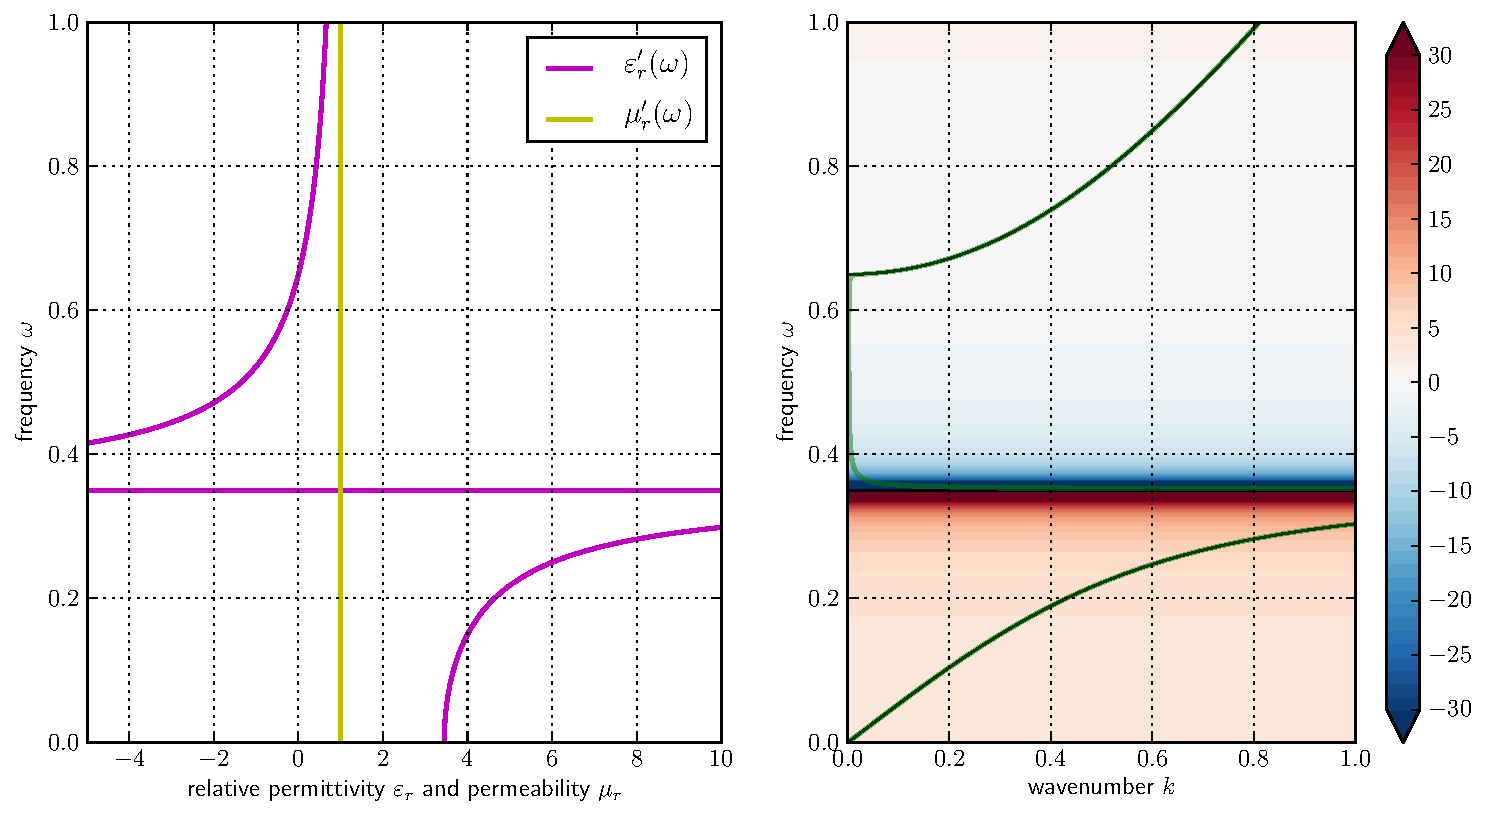
\includegraphics[width=1\textwidth]{img/dispersion_landau_lifshitz/dispersion_ll_el.pdf}    
\textbf{(b)}\\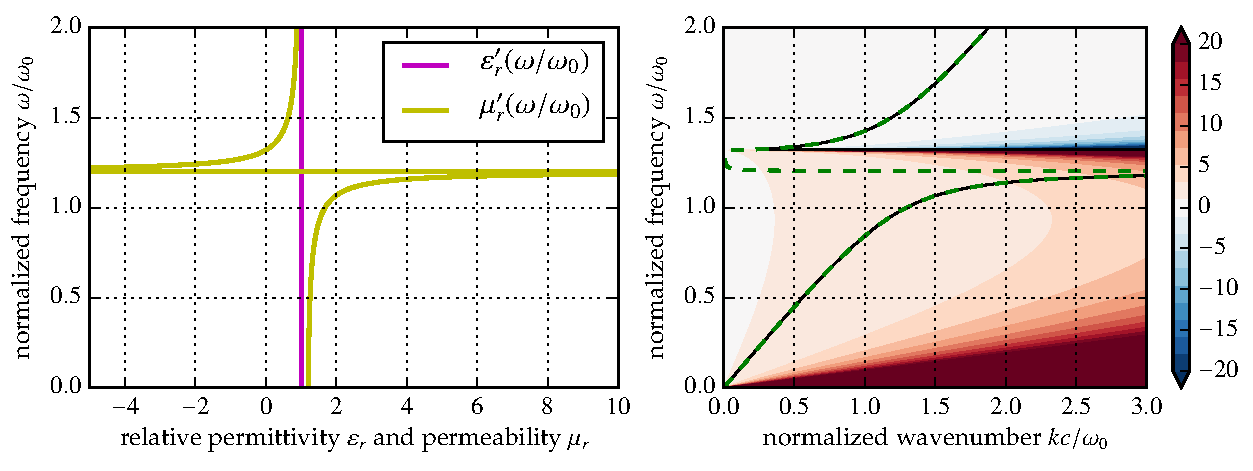
\includegraphics[width=1\textwidth]{img/dispersion_landau_lifshitz/dispersion_ll_mag.pdf}
\textbf{(c)}\\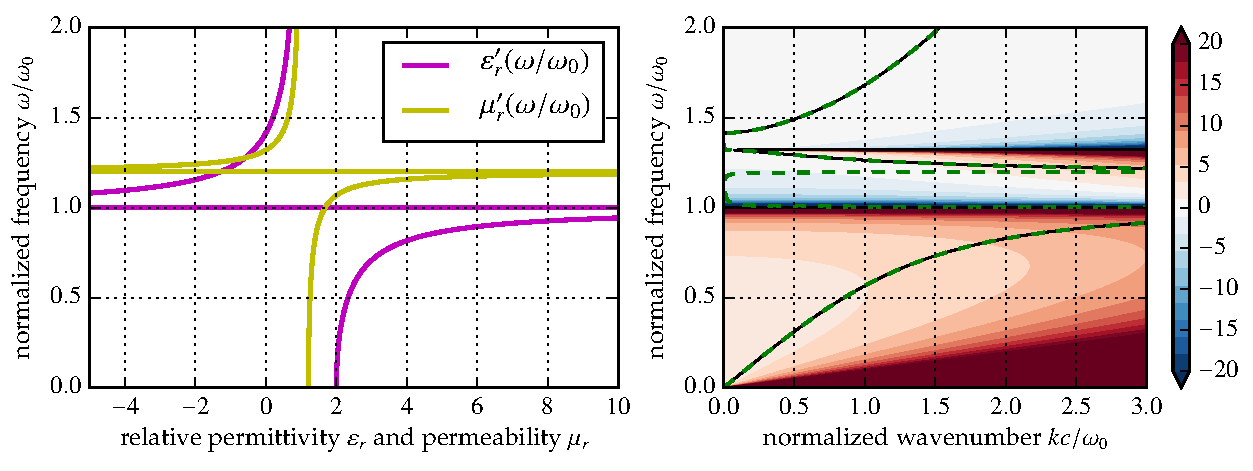
\includegraphics[width=1\textwidth]{img/dispersion_landau_lifshitz/dispersion_ll_elmag.pdf}
\end{figure}
\clearpage

The dispersion curves predicted by the classical and Landau-Lifshitz representations of the constitutive parameters for local media in Eq. (\ref{eq_epsmusd3}) are mathematically identical. This is illustrated by Fig. \ref{fg_dcll} on three examples: of a medium with (\ref{fg_dcll}a) an electric resonance, with (\ref{fg_dcll}b) a magnetic resonance and (\ref{fg_dcll}c) with both resonances overlapping. 

The plots in the left column in Fig. \ref{fg_dcll} show the \textit{local} permittivity $\epsrl(\omega)$ and permeability $\murl(\omega)$.
Its right column features a thin black contour connecting all points where the dispersion equation (\ref{eq_dispdetLL}) was found to hold by a numerical search.
This is complemented by the Landau-Lifshitz permittivity $\epsLL(\omega, k)$ as a background colour map with blue tone for negative values and red for positive ones. 
%As a confirmation of the compatibility of the Landau-Lifshitz model with the classical one,
Additionally, the original green dispersion curve as in Fig. \ref{fg_dcsimpleel} is retained, which was computed using the classical approach based on the Eq. (\ref{eq_dispeq_loc}). It can thus be seen that both models always predict exactly the same dispersion.

For a local isotropic medium with a single electric resonance in Fig. \ref{fg_dcll}a, the curves plotted are identical to Fig. \ref{fg_dcsimpleel}. On the right panel, the Landau-Lifshitz permittivity $\epsLL(\omega, k)$ follows a resonance curve in frequency, but is independent of the wavenumber $k$ (as long as the medium is local). With frequency increasing, the lower polariton branch bends towards higher $k$, as $\epsLL(\omega, k)$ increases towards the resonance at $\omega_0$, then a band of frequency follows where and no solution of the wave equation %% TODO REF
exists due to $\epsLL(\omega, k)$ being negative, and finally the upper polariton branch starts when $\epsLL(\omega, k)$ crosses zero and becomes positive again.

A local medium with a single \textit{magnetic} resonance, Fig. \ref{fg_dcll}b, is predicted by the symmetric model to exhibit similar dispersion curves. At the right panel of Fig. \ref{fg_dcll}b, the magnetic resonance is represented by the
%%% TODO add Eq. 2.52 repeated with underbrace
contribution that grows proportionally with $k^2$, and its maximum magnitude is located at the frequency $\omega_{mp}$ where $\murl(\omega_{mp}) = 0$. This shape of $\epsLL(\omega, k)$ causes the lower polariton branch to bend and approach a horizontal asymptote, which is again separated by a band of no allowed wave from the upper polariton branch, starting at $\omega_{mp}$.
$\epsLL(\omega, k)$

Finally, in Fig. \ref{fg_dcll}c, both resonances are combined. The main difference from the cases of isolated resonances occurs in the frequency range where originally $\epsLL(\omega, k) < 0$ and no wave could propagate. However, the magnetic resonance increases $\epsLL(\omega, k)$ by a term proportional to $k^2$, and consequently a new photonic branch is formed with $\mathrm{d}\omega/\mathrm{d}k < 0$, that is, with opposite group and phase velocities. IFCs for the new band then appear as sketched in Figs. \ref{fg_ifcnr}b and \ref{fg_ifcnrk}b.
% (electric quadrupoles..., [Merlin])

\todo{Why magnetic resonances do not contribute to the static permeability?}

%}}}
\paragraph{The dispersion of nonlocal media} %{{{ 
\begin{figure}[t] \caption{Dispersion curves for two nonlocal media. They differ by the value of the fourth-order expansion coefficient $\alpha(\omega)$, which was plotted with a thin blue line. The left and right columns of plots show the same information as in Fig. \ref{fg_dcll}.  } \label{fg_dcll_nl} \centering  
\textbf{(a)}\\	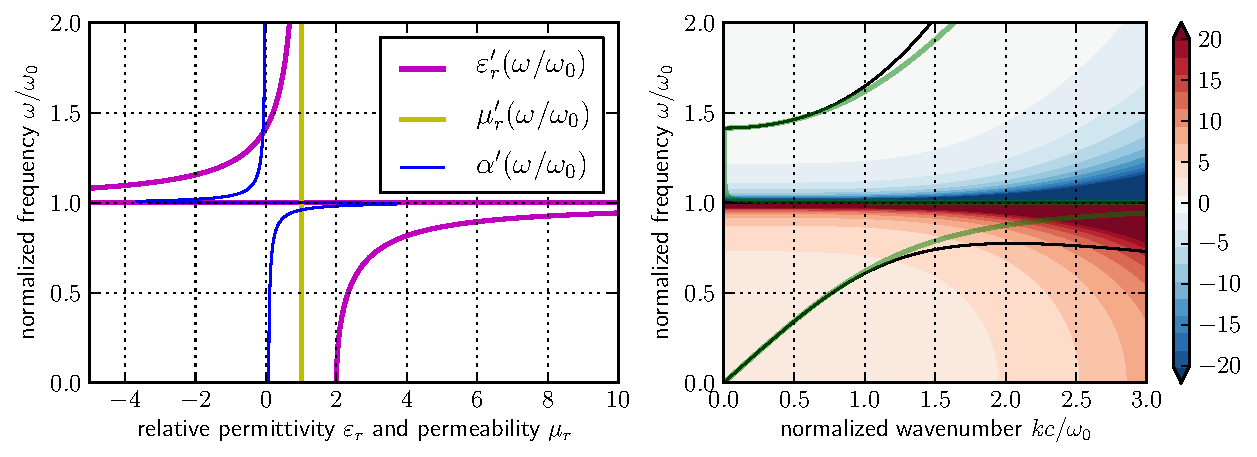
\includegraphics[width=1\textwidth]{img/dispersion_landau_lifshitz/dispersion_ll_quadrupp.pdf}
\textbf{(b)}\\	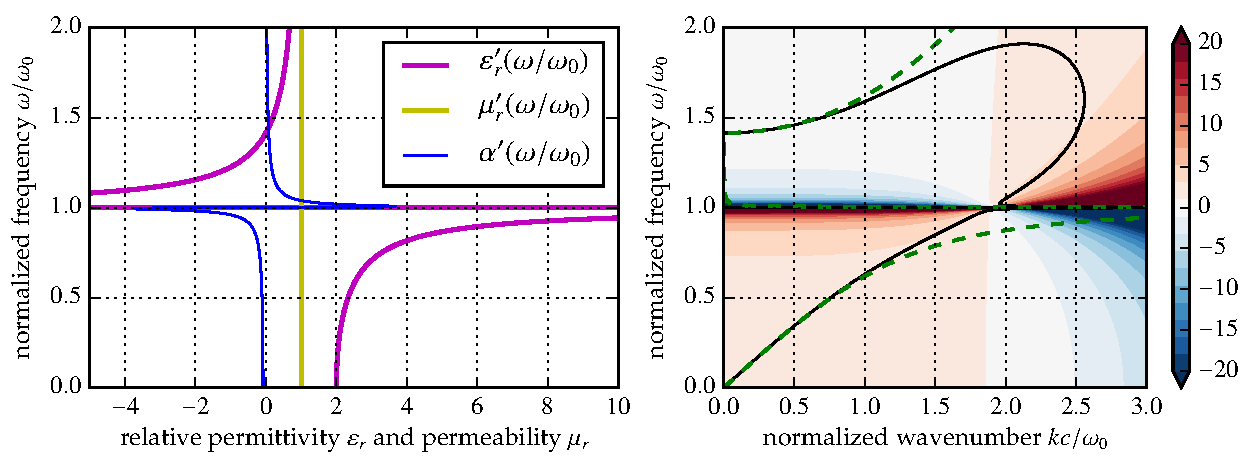
\includegraphics[width=1\textwidth]{img/dispersion_landau_lifshitz/dispersion_ll_quadrupn.pdf}
\end{figure}

Further terms in the permittivity $\epsLL(\omega,\kk)$ expansion in Eq. \ref{eq_epsmusd3} lead the dispersion curves to deviate from those predicted for local media. This corresponds to the black contour deviating from the green line in Fig. \ref{fg_dcll_nl}.
As the simplest example we add one scalar term $\alpha(\omega) k^4$ to $\epsLL(\omega,\kk)$ in Eq. (\ref{eq_epsmusd1}). The shape of $\alpha(\omega)$  was chosen as a weak Lorentz oscillator at the resonance frequency of the ordinary electric response $\chi_e(\omega)$. This is reflected in adding a thin blue line in the left column.
The choice of using the same resonance frequency for $\chi_e(\omega)$ and $\alpha(\omega)$ is not arbitrary; it is assumed that both terms arise from the same resonance mode.
\todo{+relation of higher-order terms to multipoles;  }

The choices of positive amplitude (Fig. \ref{fg_dcll_nl}a) and a negative one (Fig. \ref{fg_dcll_nl}b) have characteristic impacts on the dispersion curves. In the former case, both polariton branches deviate away from each other. In the latter case, they approach to each other with growing $k$. Eventually, in the upper right corner of the right plot in Fig. \ref{fg_dcll_nl}b, they merge into one loop. Author however believes this merging may not be observed in nature, and that its occurence is only due to unrealistic values of the $\alpha(\omega)$ coefficient, and absence of higher-order expansion terms.

%}}}
\paragraph{Multiple waves and additional boundary conditions}   %{{{ TODO
For both cases shown in Fig. \ref{fg_dcll_nl}, it is obvious the dispersion equations allow multiple solutions with different wavenumber $k$ at one frequency $\omega$. (In contrast, the existence of multiple solutions with different $\omega$ for a given wavevector $\kk$ has already occured as a usual consequence of frequency dispersion even in local media.)

The waves propagating with the higher wavenumber $k$ are denoted as \textit{additional} waves, and were predicted \cite{agranovich2006spatial, agranovich2004linear, krowne2007book, agranovich1962crystal} to be observed in natural media, e.g. near exciton levels. In the case of a positive amplitude of $\alpha$, the additional wave of the lower polariton branch has again an opposite sign of the wavevector and the group velocity ($|\vg| = \mathrm{d}\omega/\mathrm{d}k < 0$).

%}}}
\paragraph{Odd expansion terms and optical activity }   %{{{ TODO
Returning to the power expansion of $\epsLL(\omega, \kk)$ in terms of $k$ in Eq. (\ref{eq_epsmusd1}), we can identify the term constant in $k$ with the electric dipole moment $\chi_e(\omega)$, the term proportional to $k^2$ with the magnetic dipole moment $\chi_m(\omega)$ (or, also the electric quadrupole moment), and the recently discussed term proportional to $k^4$ with an electric octupole or magnetic quadrupole (\cite{agranovich2006spatial, agranovich2004linear, krowne2007book}).

The odd terms were not discussed yet, although they have important physical meaning. Their nonzero values break the spatial inversion symmetry of the medium, and are related to optical activity. In media with nonzero odd terms
, the eigenwaves are circularly polarized, and they propagate with different velocity, feeling opposite signs of the odd expansion terms. Thus, the two plots in the right column of Fig. \ref{fg_dcllactivity} can also be viewed as the dispersion curves of the same medium, for the left and right circularly polarized waves.

\begin{figure}[t] \caption{Dispersion curves for two media with optical activity. The left and right columns of plots show the same information as in Figs. \ref{fg_dcll} and \ref{fg_dcll_nl}. The frequency dependence of the term $\gamma_e(\omega)$ that is linearly proportional to $k$ in the expansion (\ref{eq_epsmusd1}) is plotted in the left column as a thin red line. } \label{fg_dcllactivity} \centering  
\textbf{(a)}\\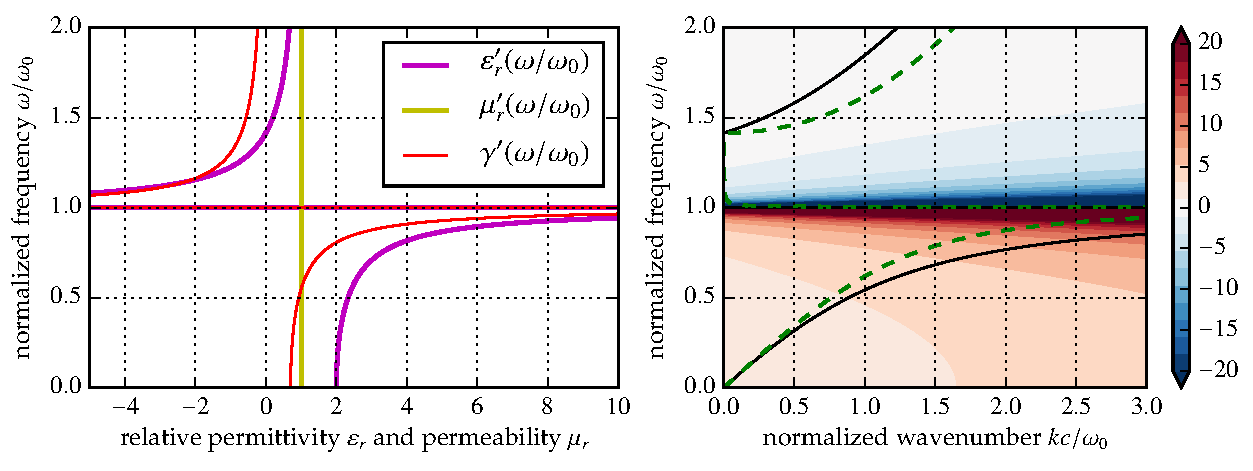
\includegraphics[width=1\textwidth]{img/dispersion_landau_lifshitz/dispersion_ll_activep.pdf}
\textbf{(b)}\\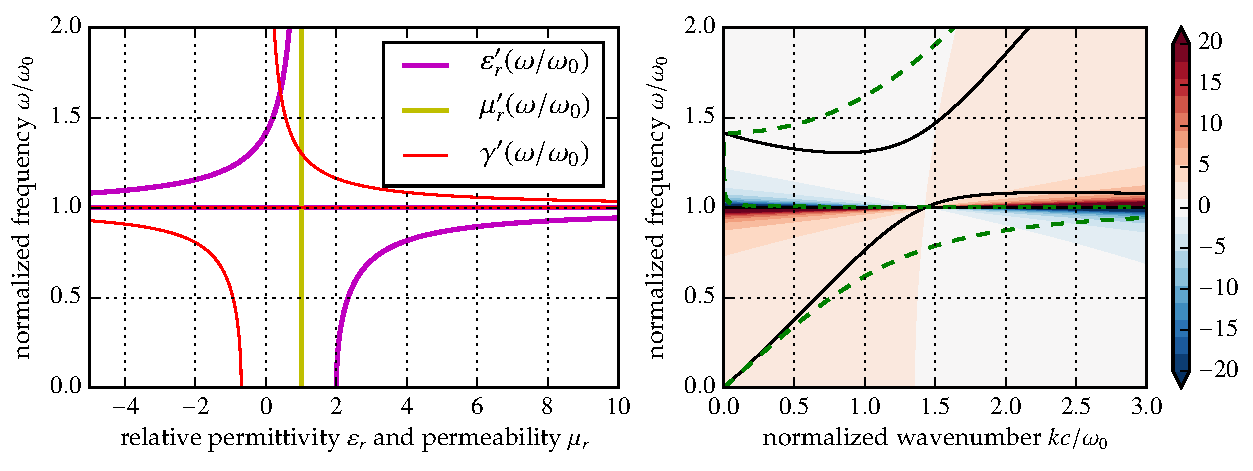
\includegraphics[width=1\textwidth]{img/dispersion_landau_lifshitz/dispersion_ll_activen.pdf}
\end{figure}

%}}}

\subsection{Impedance and amplitudes of the refraction and reflection}
\paragraph{The interface of two local media} %{{{ 
In the previous text, only the phase-related phenomena were discussed and the dependence of the dispersion curves and IFCs was computed as a result of the local or nonlocal response of the medium. Geometrical arguments then were used to infer the angle of refraction at the interface of two media, showing e.g. that a positive or negative refraction may occur, that the beam may refract in a different direction than the wave vector, and that in some cases the notion of index of refraction can be used to simplify the problem to a mere substitution into the Snell law.

The conservation of the wave phase at the interface is, however, not the only constraint to the refraction/reflection problem. Assuming there is no surface current nor surface charge, and that the medium is local, the \textit{parallel} component of the fields $\E$, $\HH$ with regards to the interface must be continuous. Additionally, the \textit{perpendicular} component of the displacements $\D$, $\B$ is continuous, too. This can be deduced from the Maxwell equations [Eq.  (\ref{eq_me1}--\ref{eq_me4})], integrating them over infinitesimally thin loops or surfaces, respercively, that are cut in half by the interface \cite[pp. 26-29]{klingshirn2007semiconductor}. 

The reflection and refraction (i.e. transmission) coefficients are derived in many textbooks  with different levels of generalisation.  
In the particular case where wave perpendicularly impinges the interface of two isotropic local media, described by their impedances $Z_1, Z_2$, respectively, the (complex) reflection $r$ and transmission $t$ are
\begin{equation} r = \frac{Z_2 - Z_1}{Z_2+Z_1}, \quad t = \frac{2 Z_2}{Z_2 + Z_1}, \label{eq_reflection}\end{equation}
with the impedances
$Z_{12} = \sqrt{\frac{{\murl}_{12}}{{\epsrl}_{12}  }  }$.
This is in fact similar to the reflection on a one-dimensional transmission line, as known from the microwave engineering.

If the incidence is not perpendicular, the complex amplitudes of the reflected and transmitted wave depend on the angle of incidence, and splits into the TE and TM polarisation \cite[p. 38]{born1999book}.

%}}}
\paragraph{Refraction on interface with a nonlocal medium}   %{{{ TODO
-

\add{
Extending the notion of impedance to spatial-dispersive media to compute the  amplitudes. 
The reason lies in the spatial-dispersive media always being assumed infinite, so their interfaces are not accounted for in the model. If such an extension would be done, the spatial integral in Eq. \ref{eq_eq_chi_convol_nonloc} would have to be better specified, either with the nonlocal response of medium to extend also behind the interface. Alternatively, the medium response could be sharply truncated at the interface.
}

\todo{add from \cite{golubkov1995boundary}}

%}}}


\subsection{Phase, group, energy and signal velocity}
\paragraph{Sign of the phase and group velocities}%{{{ TODO
The negative refraction in media shown in Figs. \ref{fg_ifcnr}b,c and \ref{fg_ifcnrk}b,c was a result of the requirement for the group velocity $\vg$ to maintain its component perpendicular to the interface, and for the wave vector $\kk$ to maintain its projection onto the plane of interface. Therefore, in media with low losses, the term of negative refraction 

\add{... in media with time reversal, the wave may always propagate backwards - we should always speak of mutual sign of the velocities}

phase velocity is often higher than the speed of light, this is no problem\\

%}}}
\paragraph{"Negative-refraction", "negative-index", "left-handed" or "doubly-negative" media?}  %{{{
Media with a negative index of refraction are a subset of negative refraction, where the notion of index of refraction makes sense, as discussed above.

\add{When the index of refraction $N = \sqrt{\epsrl\murl}$ and the impedance $Z = \sqrt{\frac{\murl}{\epsrl}}$ are both defined, one may easily deduce that 
\begin{equation} \epsrl = \pm\frac{N}{Z}, \quad \murl = \pm N\,Z. \label{eq_nzepsmu}\end{equation}
The question of indefinite sign can be decided using the assumption of medium \textit{passivity}, that is, of the medium absorbing the wave rather than amplifying it. \todo{describe further}

\todo{ (here first cite Veselago, not earlier, not later, note that Veselago68 speaks about a truly *homogeneous* medium)\\ }

\todo{add the comments from http://www.wave-scattering.com/negative.html}
}
%}}}
\paragraph{Sign of the group and energy velocities}  % TODO %{{{
%  \mdf{
%  % TODO 0401 how can one tell apart negative refraction due to eps-mu and due to higher, purely nonlocal terms?
%  *doubly resonant local media -> negative phase velocity, positive group velocity, above resonant frequencies - theoretically arbitrarily small losses\\
%  *singly resonant local media -> positive phase velocity, negative group velocity, this happens near resonance so there are always high losses\\
%  *			  nonlocal media -> weird things happen, todo\\
%  }
In the discussion of wave refraction on an interface, it was assumed that the envelope (or modulation) of the wave approaches the interface in the first medium, then refracts and propagates out \textit{from} the interface in the second medium. The envelope propagates with the group velocity, $\vg$, as defined by Eq. (\ref{eq_vg}). There is another quantity, the \textit{Poynting vector} $\mathbf{P} := \E\times\HH$, describing the direction and density of the \textit{power} carried by the optical wave. \todo{cite}

The group velocity usually points in the same direction as the Poynting vector, but this has not necessarily to be always true. A typical counterexample can be found near resonances in lossy (local) media. Such a behaviour can be traced back to Fig. \ref{fg_oscillator_spectrum}, where the permittivity drops from high values to negative ones. If the medium is defined as a lossy one, the curve of the wavenumber $k(\omega)$ is continuous and smooth, and as a result the magnitude of the group velocity $v_g = \mathrm{d}\omega / \mathrm{d}k$ is negative around the resonance for $\omega \sim 2\pi$, %% TODO "negative" means "opposite to kk"? But we are speaking of scalars...
which is also known as \textit{anomalous dispersion}. 

It follows from this that the group velocity $\vg$ can also point opposite to the Poynting vector that represents propagation of the light beam energy, $\mathbf{S}$. 
% This fact can not be easily deduced from the dispersion curves or IFCs. %% TODO  Or can it?
This behaviour can be observed in narrow parts of the spectrum only, around the resonance frequencies where the media have high losses, and also a strong group velocity dispersion.
Assuming passivity and absence of sources in the second medium, it is obviously the Poynting vector that has to maintain its perpendicular component and that the group velocity   inevitablyhas to point towards the interface also in the second medium, which seems contradictory to causality.
This result 
%of the light envelope propagating with the group velocity \textit{from} the second medium \textit{towards} the interface may seem unphysical, 
may however be explained through strong deformation of the envelope shape on a short distance, which ensures the information carried by the wave modulation to propagate causally, out from the source, and always with speed lower or equal to the speed of light in vacuum, $c$.

Negative group velocity has been experimentally observed in a thin sample. It manifested as a negative shift of the light envelope compared to the absence of the medium \cite{dolling2006simultaneous}. Note that the negative group velocity is independent of the sign of the phase velocity, which may be both positive and negative \cite{mikki2009electromagnetic}.

%}}}
\paragraph{Signal velocity}%{{{
The notion of \textit{signal} or \textit{information propagation velocity} is sometimes % TODO cite
identified with the group velocity, $\vg$. However, this may be misleading, as its differential definition in Eq. (\ref{eq_vg}) enables one to define the group velocity for slow-enough modulation only, so that the span of frequencies is narrow and the second derivative, corresponding to the group velocity dispersion, can be neglected.

%In the author's view, it is rather a problematic term because a 
Assuming the information is carried by a wave modulation that is limited in time (e. g. presence or absence of an optical pulse), leads to a contradiction. From the convolution-multiplication theorem already used in Eq. (\ref{eq_kkresult}), it can be shown that any information carrying function with a finite-support has to span over an infinite spectrum. 
A temporally limited optical pulse will be always more or less distorted upon propagation in dispersive medium, and the information velocity becomes a problematic term.
Therefore, the author is convinced that \textit{information} velocity can not be directly identified with the group velocity. 

%}}}
%% TODO \paragraph{Speed of light and causality in spatial-dispersive media}%{{{
%% \mdf{TODO REF Kramers-Kronig relations in nonlocal medium
%% \cite{skettrup1970kramers}
%% \cite{kirzhnitz1976}
%% \cite{melrose1977generalised}
%% \cite{sun1989kramers}
%% \cite{rozanov2003}
%% \cite{bruleanalysis}
%% \cite{makarov2013kramers}
%% }%}}}
%% 

\section{Electromagnetic waves in periodic structures}
\subsection{Periodic structures and the Bloch-Floquet theorem}
\paragraph{Periodicity}%{{{
The previous sections discussed infinite homogeneous media. The only exception was when a refraction at an interface of two media was discussed, for which we shown that the possible orientation of the wave vector and of the group velocity could be easily deduced on geometrical basis. The amplitude of the reflected and refracted waves can be also easily computed for local media, whereas their computation for nonlocal media is much less straightforward. 

There is a broader class of structures for which analytical or semianalytical methods have been developed to compute their interaction with electromagnetic waves, such as scattering on dielectric/metallic spheres, propagation through arbitrary stacks of parallel layers, diffraction on thin apertures, resonances in orthogonal, cylindrical or spherical cavities, or wave guiding in high-symmetry waveguides or optical fibers. 

The interaction of electromagnetic waves with the rest of possible structures is generally too complex to be expressed analytically, and can only be accessed by numerical methods, some of which are described in the Chapter \ref{chapter_numerical}. However, when these elementary structures are arranged into an infinite array, the resulting structure behaves in a way that is characteristic for the periodicity and its most important traits can again be partially understood on analytical basis.

In this chapter, we will focus on these general properties of periodic structures, leaving the particular numerical simulations to the Results section.
Under the notion of \textit{periodicity} we understand there exist discrete translational symmetries, that is, 
\begin{equation} \epsrl(\omega,\rr) = \epsrl(\rr + m_1 \mathbf{a}_1 + m_2 \mathbf{a}_2 + m_3 \mathbf{a}_3) \quad\text{(in three dimensions).} \label{eq_trsym}\end{equation}
where $m_1, m_2, m_3 \in \mathbb{Z}$ and $\mathbf{a}_1, \mathbf{a}_2, \mathbf{a}_3$ are three linearly independent vectors. The \textit{local} relative permittivity, given by Eq. (\ref{eq_lorentz_eps}), was intuitively generalized to a function of the position $\rr$. Note that only the local quantities are used to avoid possible problems at the boundary computing the spatial convolution [Eq. (\ref{eq_eps_nonloc})]  in nonlocal media. The same expectation is also imposed at the permeability $\murl(\omega,\rr)$. 

The points generated by all combinations of possible translations by $m_1 \mathbf{a}_1 + m_2 \mathbf{a}_2 + m_3 \mathbf{a}_3$ form a periodic lattice.
The minimum volume associated to each point of the lattice will be denoted as a \textit{unit cell}. Obviously, the permittivity or permeability in periodic structures needs only to be specified in the domain of one unit cell.

In three dimensions, there are six \textit{crystal families} that differ rotation or mirror symmetries of their lattices, namely \textit{cubic}, \textit{tetragonal}, \textit{ortorhombic}, \textit{monoclinic}, \textit{hexagonal/trigonal} and \textit{triclinic}. Combined with all possibilities for the symmetry of the permittivity and permeability distribution in each unit cell, the periodic structures can be classified into total 230 \textit{crystallographic point groups} in three dimensions. Numerous crystal optics textbooks (e.g. \cite[p. 678]{born1999book}) give more rigorous definitions. % based on the group theory. 
Unless stated otherwise, we will assume the cubic lattice is used, which has highest possible symmetry. In the cubic lattice, $\mathbf{a}_1, \mathbf{a}_2, \mathbf{a}_3$ are of the same magnitude and mutually orthogonal. Note however that no structure with a periodic modulation of permittivity is truly isotropic, i.e. posessing continuous rotational symmetry.

%}}}
\paragraph{The Bloch theorem}%{{{
The \textit{Bloch-Floquet theorem} states that while the wave in a periodic structure (see. Eq. \ref{eq_trsym}) does not have to be periodic anymore, it can always be expressed a product of two periodic functions:
\begin{equation} 
\E(t, \rr) = \mathbf{u_e}(\rr)\,\mathrm{e}^{\ii\omega t - \ii\KK\cdot\rr}, \text{ where } \mathbf{u_e}(\rr) = \mathbf{u_e}(\rr + m_1 \mathbf{a}_1 + m_2 \mathbf{a}_2 + m_3 \mathbf{a}_3).
\label{eq_bloch}\end{equation} 
\begin{equation}
\HH(t, \rr) = \mathbf{u_m}(\rr)\,\mathrm{e}^{\ii\omega t - \ii\KK\cdot\rr}, \text{ where } \mathbf{u_m}(\rr) = \mathbf{u_m}(\rr + m_1 \brho_1 + m_2 \brho_2 + m_3 \brho_3).
\label{eq_blochh}\end{equation} 
Thus, $\mathbf{u_e}(\rr)$, $\mathbf{u_m}(\rr)$ have the same periodicity as the structure, and will be denoted as the \textit{mode functions}. They are generally complex vector functions, so they not only alter the direction and magnitude of the electric and magnetic fields, but can also introduce a \textit{phase modulation} of the wave in each unit cell. 

The remaining term, $e^{\ii\omega t - \ii\KK\cdot\rr}$, is formally identical to that of a plane wave
\begin{equation} \E(t, \rr) := \E_0\, e^{\ii\omega t - \ii\kk\cdot\rr}, \tag{\ref{eq_pw} \again} \end{equation}
except for the capital $\KK$ being used to distinguish the wave vector of the Bloch wave envelope from the wave vector $\kk$ in homogeneous media. 

Note this theorem does not determine the shape of $\mathbf{u_e}(\rr)$, $\mathbf{u_m}(\rr)$, nor the direction and magnitude of $\KK$, it only states a solution in the form of Eqs. (\ref{eq_bloch}, \ref{eq_blochh}) can be found.
% TODO proof /home/filip/PhD/Sources_MM_theory/Bloch_Theorem_Proof.pdf
% TODO example illustration of Bloch wave -> plotted in Python

%}}}
\paragraph{The proof of the Bloch-Floquet theorem}%{{{
This theorem is essential for understanding the electromagnetic behaviour of periodic structures, and it deserves a proof. Originally, it was developed for the electron wave function $\psi$ in crystals on the basis of quantum mechanics. The outline of the proof which is the most often found in textbooks (e.g. \cite[p. 134]{ashcroft2005solid}) is based on the following:
\begin{enumerate}
 \item{We assume $\psi$ is an eigenfunction of the Hamiltonian: $\exists h\in \mathbb{C}: \hat H\psi = h\psi$.} 
 \item{We also assume that the Hamiltonian operator $\hat H$ commutes with the operator of discrete translation $\hat T$ by the inter-atomic distance: $\forall \psi: \hat H\hat T\psi = \hat T\hat H\psi$ } 
 \item{Then $(T\psi)$ is an eigenfunction of $H$, because obviously $\hat H(\hat T\psi) \stackrel{1.}{=} \hat T\hat H\psi \stackrel{2.}{=} \hat Th\psi = h(\hat T\psi)$.}
 \item{From two eigenfunction relations, $\hat H\psi\stackrel{2.}{=} h\psi$ and $\hat H(\hat T\psi) \stackrel{3.}{=} h(\hat T\psi)$, it also follows that 
$\exists K\in \mathbb{C}: \hat T\psi = e^{-\ii Ka}\psi$. \todo{cite} Therefore, eigenfunction $\psi$ is repeated across the cells, differing only by the phase being multiplied by $-Ka$. Setting $a$ to be the unit cell size, $K$ becomes the wavenumber of the Bloch wave envelope.
%$\exists t\in \mathbb{C}: hT\psi = HT\psi = Ht\psi = ht\psi$. \todo{cite} %In the special case that more eigenfunctions are associated 
}
 \end{enumerate}
% As can be easily shown, two commuting operators share the same eigenstates, which means that the electron wave function at a given energy (i.e. Hamiltonian eigenfunction) must also have a discrete translational symmetry provided its phase can change between atoms (i.e. it is an eigenfunction of the non-hermitian translation operator).
The steps will be followed using the explicit, classical formulation of electromagnetism as the rest of this thesis does. We can no further assume the solution in the form of a plane wave (\ref{eq_pw}), but as long as the structure is time-invariant and linear, the electric and magnetic fields can still be decomposed into monochromatic components:
\begin{equation} 
\begin{array}{cc}
\E(t, \rr) = \E(\rr) e^{\ii \omega t}, \\
\HH(t, \rr) = \HH(\rr) e^{\ii \omega t}. 
\end{array}
\label{eq_harmonic}\end{equation}
We thus only need to prove the Bloch theorem for the time-invariant parts of the fields, which will play the same role as the wavefunction $\psi$.

\begin{enumerate}
\item{
For $\E(\rr)$ to be a  valid solution of Maxwell equations in the periodic structure at the angular frequency $\omega$,
it can be derived from Eq. (\ref{eq_me3}, \ref{eq_me4}, \ref{eq_epstensor} and \ref{eq_harmonic}) in straightforward manner that
\begin{equation} 
{\epsrl}^{-1}(\omega,\rr) \nabla\times \left[{\murl}^{-1 }(\omega,\rr) \nabla\times \E(\rr) \right] = \frac{\omega^2}{c^2}\E(\rr),   \label{eq_eigen_e}
\end{equation}
In analogy with the quantum-mechanical proof, the left hand side of Eq. (\ref{eq_eigen_e}) can be associated with the Hamiltonian $\hat H\psi$, and the right hand side with its eigenvalue $h\psi$. Obviously the operator differs for the electric and magnetic field.
} 
\item{
The translation operator acts by substitution of the position vector $\rr$, e.g. for the electric field:
\begin{equation} \hat T\psi \rightarrow \E(\rr+\mathbf{a_1}). \label{eq_blocht}\end{equation}
The commutation relation directly follows from the periodicity in Eq. (\ref{eq_trsym}), thus right terms in Eqs. (\ref{eq_blochht}) and (\ref{eq_blochth}) are equal:
\begin{equation} \hat H \hat T \psi \quad  \rightarrow \quad  {\epsrl}^{-1}(\omega,\rr             ) \nabla\times \left[{\murl}^{-1 }(\omega,\rr             ) \nabla\times \E(\rr) \right] \E(\rr+\mathbf{a_1}) \label{eq_blochht}\end{equation}
\begin{equation} \hat T \hat H \psi \quad  \rightarrow \quad  {\epsrl}^{-1}(\omega,\rr+\mathbf{a_1}) \nabla\times \left[{\murl}^{-1 }(\omega,\rr+\mathbf{a_1}) \nabla\times \E(\rr) \right] \E(\rr+\mathbf{a_1}).  \label{eq_blochth}\end{equation}
In three dimensions, the argument is to be repeated for three different translation operators that correspond to the addition of the different lattice vectors, $\mathbf{a_1}$, $\mathbf{a_2}$ and $\mathbf{a_3}$.
} 
\item{
Then the wave translated by any of the lattice vectors $\mathbf{a_1}$, $\mathbf{a_2}$ and $\mathbf{a_3}$ is also a solution of Maxwell equations:
\begin{equation}  {\epsrl}^{-1}(\omega,\rr) \nabla\times \left[{\murl}^{-1 }(\omega,\rr) \nabla\times \E(\rr) \right] \E(\rr+\mathbf{a_1}) =  \frac{\omega^2}{c^2}\E(\rr+\mathbf{a_1}).  \label{eq_blochth}\end{equation}
}
\item{
\begin{equation}  \E(\rr+\mathbf{a_1}) = e^{-\ii K_1 a_1} \E(\rr),  \label{eq_blochtt}\end{equation}
where $K_1 a_1$ represents the phase shift between the adjacent cells. \todo{discuss the $\KK$ vector further}
}
 \end{enumerate}
The same arguments have to be valid also for the magnetic field $\HH(\rr)$, where the Hamiltonian is associated with a slightly different operator:
\begin{equation}
{\murl}^{-1 }(\omega,\rr) \nabla\times \left[{\epsrl}^{-1}(\omega,\rr) \nabla\times \HH(\rr)\right] = \frac{\omega^2}{c^2}\HH(\rr).   \label{eq_eigen_h}
\end{equation}

%}}}
\paragraph{Virtual periodicity and ambiguity of the mode function}%{{{
\begin{figure}[ht] \caption{Folded and unfolded dispersion curves for free space and photonic crystal. The phase difference over an unit cell can be expressed either by the wavenumber $K$ (unfolded plots \textbf{a, b} above), or it can be partially absorbed into the periodic mode function $\mathbf{u}(\rr)$ (folded plots \textbf{c, d} below) } \label{fg_phc} \centering  %% TODO write caption; complement the text to match
	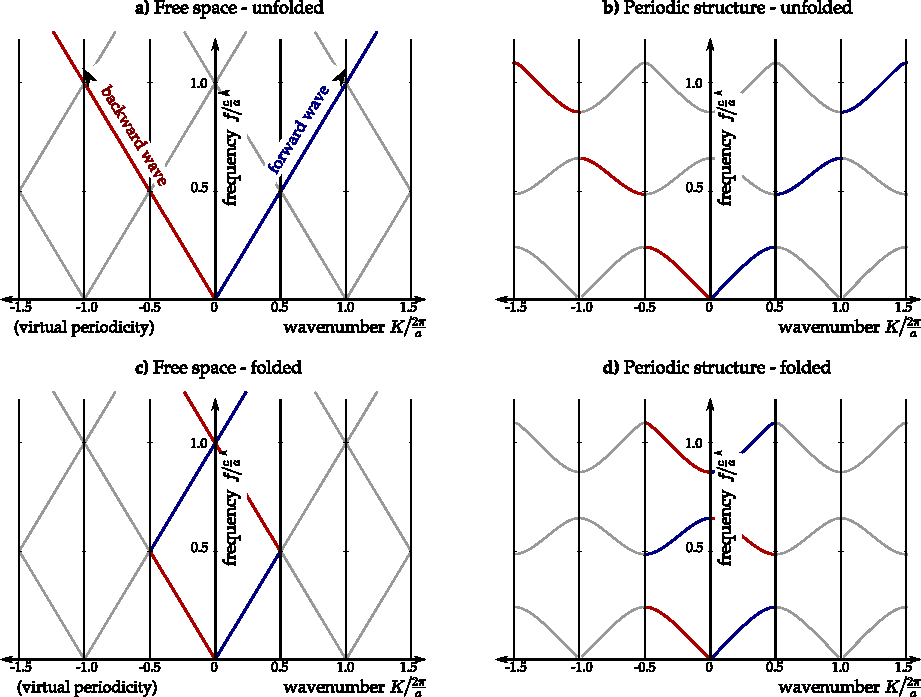
\includegraphics[width=\textwidth]{img/PhC_folding_illustration.pdf} 
\end{figure}
Homogeneous media, such as vacuum, naturally fulfill the definition of periodicity in Eq. (\ref{eq_trsym}).
From the principle of correspondence, the predictions of the Bloch-Floquet theorem should be verified against the already known solution of a plane wave in vacuum, 
\begin{equation} \E(t, \rr) := \E_0\, e^{\ii\omega t - \ii\kk\cdot\rr}. \tag{\ref{eq_pw} \again} \end{equation}
One solution of the Bloch wave in vacuum can be directly found as a formal modification of the dispersion relation,
\begin{equation}  
\E(t, \rr) = \mathbf{u_e}(\rr)\,\mathrm{e}^{\ii\omega t - \ii\KK\cdot\rr}, \text{ where } \mathbf{u_e}(\rr) := \E_0  \text{ and } \KK := \kk.
\label{eq_blochvac}
\end{equation}
Any lattice of periodic unit cells may be imagined in vacuum. With an arbitrary choice of the unit cell size $a$, % TODO represent by lattice vectors G?
the plane wave in vacuum can be also represented by any of infinitely many other combinations of
\begin{equation} 
\left.  \begin{array}{cc}
\mathbf{u_{e}}(\rr) := \E_0 e^{2\pi\ii (m_1/a_1 + m_2/a_2 + m_3/a_3)} \\
\KK := \kk - \frac{2\pi m_1}{a_1} - \frac{2\pi m_2}{a_2}- \frac{2\pi m_3}{a_3},
\end{array}\quad \right\} \quad \forall m_{1,2,3} \in \mathbb{Z}
\label{eq_blochvac2}
\end{equation}
which all maintain the requirement of the mode function $\mathbf{u_{e}}(\rr)$ being periodic and still give the exactly same resulting plane wave.  \todo{inconsistent use of vector-3D and one-dimensional approach, discuss}

All possible dispersion curves for a Bloch wave with the $\KK$ vector oriented along one lattice axis in vacuum is plotted in Fig. \ref{fg_phc}a. The dispersion curve for the original forward wave from Eq. (\ref{eq_blochvac}) is plotted in blue; another solution exists for a wave propagating in the opposite direction which is plotted in red. All other solutions generated by Eq. (\ref{eq_blochvac2}) are plotted in gray, for both forward and backward waves. 

Note that the actual physical shape of the fields in space can not be deduced from the dispersion curve. To fully determine it, the dispersion curves would have to be complemented by the mode functions $\mathbf{u_e}(\rr)$ and $\mathbf{u_m}(\rr)$. This leads to the inherent ambiguity of description on the basis of the Bloch wave, which can be used to graphically save space in the plot by showing the dispersion curves only for $K\in\langle-\pi/a, \pi/a\rangle$, as shown in Fig. \ref{fg_phc}c. Plotting any other interval of equal width would be equivalent. 

xx-alibaba
xx_babylon

fgbabylon

Further, all forward and backward propagating solutions are mirror-symmetrical with respect to the vertical $K=0$ axis, except for structures with optical activity (c.f. Fig. \ref{fg} or even breaking the time-reversal symmetry (c.f. \cite{vanwolleghem2009unidirectional}). Thus, in many papers on periodic structures \todo{cite some!}
, all dispersion curves are \textit{folded} in the $K\in\langle0, \pi/a\rangle$ region only. In some other papers, full unfolded dispersion curves are used.

The physical interpretation of folding 

The lattice periodicity allows to draw the dispersion curves of periodic structures using natural, scale-invariant units, with the Bloch wave number $K$ divided against the spatial frequency of the lattice $2\pi/a$, and the angular frequency $\omega$ multiplied by the time needed for the light to traverse the unit cell.



\todo{rewrite?}
\add{
When the wavelength is less than double cell spacing, or equivalently when $2\pi c /K < 2 a$, the unit cells can scatter the forward propagating wave into the backward direction and vice versa. In an infinite periodic structure the energy transfer must be conserved, so the forward and backward waves must be of the same amplitude. (The equilibrium of forward and backward wave amplitudes may, however, differ in some cases even in in infinite periodic structure. One example is when the constituent materials lose time-reversal symmetry due to static magnetic field.) We assume this also in this example with virtual periodicity. The \textit{Bloch wave} is a product of two functions, and it gives one degree of freedom to select which part of (\ref{eq_bloch}) expresses the phase shift across one unit cell. Two different conventions are used in the literature.
}


\begin{enumerate}
 \item{In the \textit{unfolded} plot, the phase shift is expressed entirely by the envelope $\mathrm{e}^{\mathrm{i}Kz}$. One can always find a line coming from the front side of a unit cell to its back side, along which the mode function does not change its phase significantly $\mathbf{u(\mathbf{r})}$. In other words, the volume of the unit cell is not divided by any \textit{nodal plane} in the real part of electric field  $\mathbf{u(\mathbf{r})}$. (However, closed nodal planes within the unit cell may appear due to individual resonances.)

In vacuum, the mode function takes the simplest form, being constant $\mathbf{u(\rr)} = 1$ at all frequencies. The dispersion relation of vacuum forms a direct line as plotted in Fig. \ref{fg_phc}a.} 
 \item{The \textit{folded} plot requires $K/\left(\frac{2\pi}{a}\right) \in (-\frac{1}{2}, \frac{1}{2})$ and the remaining phase is mostly expressed by the mode function. 
Further savings of space in the plot can be made using the symmetry of the forward and backward waves, so only the positive half for $K/\left(\frac{2\pi}{a}\right) \in (0, \frac{1}{2})$ has to be plotted to describe the mode structure.} 
\end{enumerate}
Although maybe less instructive, usually the \textit{folded} bands are plotted in the literature and they are used also in Fig. \ref{fg_1dbd}, \ref{fg_rodh} and \ref{fg_erod_radius11} below. The same approach can be used for periodic structures, where the bands are separated by band gaps, cf. Fig. \ref{fg_phc}b and \ref{fg_phc}d.

%}}}
\paragraph{Fourier expansion of the mode function}%{{{
\add{If there is a real modulation within the unit cell, the above mentioned ambiguity between accumulating the phase in the wave vector $\KK$ or in the mode $\mathbf{u}(\rr)$ gets a new meaning: the field in the unit cell can be decomposed into a Fourier sum of waves, thus defining some amplitude $a_n$ for every possible branch.

The field shape given by Eq. (\ref{eq_}) \todo{eq}
 }

%}}}
\paragraph{Reciprocal space, Brillouin zones and Isofrequency contours} %{{{ TODO

%}}}
\paragraph{}%{{{

%}}}
in the following we will plot the unfolded bands instead as it seems to give clearer physical interpretation of data.
-> TODO doplnit "PhC book": dispersní křivky atd.

A different view to the formation of the dispersion curves can be drawn in analogy with the \textit{tight-binding} model in solid-state physics, first analyzing the unit cells isolated in free space, and then taking into account their mutual interaction that shifts the frequency up, or down. \label{hopping}
The 
This is . %-- individual oscillators with frequency more-or-less dependent on

Returning to the figure of dispersion curves in a periodic structure, % TODO ref
the $\Gamma$ point in the Brillouin zone, where $k = 0$, can be identified with Neumann boundary conditions, where we require $dE/dx = 0$ (otherwise the derivative of the field $E$ would not be continuous). % this also holds for other boundaries, on the $y$- and $z$-axis

In contrast, the $X$ point, where $k_x = 2\pi/a_x$, corresponds to the Dirichlet boundary condition at the boundary perpendicular to the $x$-axis.
M-point ... "E=0")



\paragraph{}%{{{

%}}}
\paragraph{}%{{{

%}}}
\paragraph{}%{{{

%}}}
\paragraph{}%{{{

%}}}


\subsection{Properties of photonic band-gaps}
% -> application of PBG, todo add references; formation: \cite{laktionov2008}
% -> zero-width case, as a transition between a mode traversing from one photonic band to another
% -> concept of nodal planes (or, more precisely, surfaces)
% -> exponential wave decay with phase difference across the cell
% -> note about how Fourier transform allows no point source to radiate energy within the bandgap
% -> PhCs with metallic/metamaterial inclusios, [Monsoriu, Lina Shi and friends]


%  \cite{johnson2003introduction}
%  Electromagnetic wave propagation in periodic media was first studied by
%  Lord Rayleigh in 1887, in connection with the peculiar reflective properties of a
%  crystalline mineral with periodic “twinning” planes (across which the dielectric
%  tensor undergoes a mirror flip). These correspond to one-dimensional photonic
%  crystals, and he identified the fact that they have a narrow band gap prohibiting
%  light propagation through the planes. This band gap is angle-dependent


\subsection{Homogenization}
\mdf{
Homogenization is not a search for an existing truth, but rather a somewhat arbitrary decision.

Effective parameters

ref Homogenisation issues - response to our paper from OpEx
\cite{rockstuhl2008transition}
\cite{paul2011reflection}
\cite{andryieuski2012bloch}
\cite{andryieuski2010homogenization} 
\cite{simovski2007bloch}
\cite{simovski2009material}
\cite{simovski2011electromagnetic}
\cite{mortensen2010unambiguous}
}
%% "process of replacing a complex structure of subwavelength sized components with an “effective medium” with uni-
%% form properties. It is a fundamentally important notion which can be traced back to the earliest days of electro-
%% magnetic theory, to the Lorentz-Lorenz and Maxwell-Garnet effective medium models [1–3]
%			[1] J. C. M. Garnett, Phil Trans. R. Soc. A 203, 385 (1904).
%			[2] D. E. Aspnes, Thin Solid Films 89, 249 (1982).
%			[3] W. Cai and V. Shalaev, Optical Metamaterials: Fundamentals and Applications (Springer, New York, 2010).

%% Many MMs do not bring negative refraction, other (composites) do, but not by means of resonances: 
%% The tunable negative permittivity and negative permeability of percolative Fe/Al2O3 composites in radio frequency range with
%% Negative index may arise from resonances


\subsection{What are metamaterials and photonic crystals?} %{{{
\add{
%% This is after the theory of eldn in periodic media.
%% Nonresonant metamaterials (ie. in the 1st Brillouin zone, see [Kadlec2008 / Vol. 33, No. 19 / OPTICS LETTERS] and Juraj]
%% resonant metamaterials operate in the 2nd BZ (or possibly even third or higher? )
%% Think over, note the paper Dominec2014

The studies of periodic electromagnetic structures is generally divided into two classes: the \textit{photonic crystals} and \textit{metamaterials}. These types of structures are formally very similar, as they are composed of 2-D or 3-D periodic array of unit cells, and the qualitative difference can be found only after the interaction with an electromagnetic wave is known. 

%The difference is in the way how the unit cell interacts with the electromagnetic field. 

Both types of structures exhibit the most interesting behaviour at their frequencies of resonance, but the different types of resonances define the technology and materials used to build them. The resonances in PhC rely on wave scattering, which can be easily obtained with any ordinary low-permittivity material such as silica or silicon. On the other hand, the resonances 
%but the mentioned difference has profound consequences on the behaviour of the structure. 
%}}}

note silveirinha2007metamaterial \cite{silveirinha2007metamaterial}
resonant metamaterials operate in the 2nd BZ (or possibly even third or higher? )
Think over, note our paper dominec2014transition \cite{dominec2014transition}

}
\paragraph{Definition by the Bloch wavelength}
Igor Tsukerman in Ref. \cite{tsukerman2011nonlocal}: \textit{"metamaterials - artificial periodic structures with features smaller than the vacuum wavelength"} 

\begin{figure}[h] \caption{Schematic of usual relation of reciprocal lattice vector to the wavelength in metamaterials and photonic crystals}  \centering 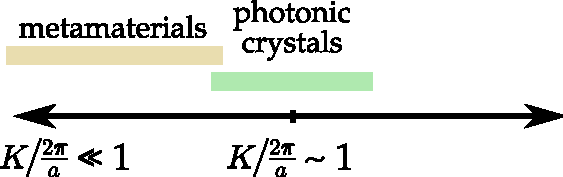
\includegraphics[width=8cm]{img/mm-phc-diagram.pdf} \end{figure} 

\add{The notion of "wavelength", or more precisely "Bloch wavelength", is not uniquenly defined in such structures! }

\paragraph{Definition by energy localisation}

\add{Energy is the most localized at the frequencies of resonances.}

In the photonic crystal (PhC), at its frequency range of operation, the effective wavelength is similar to the cell spacing and the cells scatter the propagating wave.
The energy of the resonant field is spread relatively evenly over the majority of the unit cell volume, which results in great sensitivity of the PhC behaviour to its periodicity and typically also in a high spatial dispersion. The most prominent phenomenon observed in PhC is the emergence of forbidden photonic bands around resonant frequencies, where the light can not propagate through the structure. 

On the contrary, the cells of a metamaterial (MM) are expected to exhibit individual resonances which should not significantly couple to each other. 
At the resonant frequencies in the metamaterials, the majority of the energy of the electromagnetic field is localised in a fraction of the unit cell volume, so that the behaviour of the metamaterial usually has only weak spatial dispersion, if any. This allows one to describe many metamaterials with acceptable precision as a homogeneous medium with a index of refraction $N(f)$, wave impedance $Z(f)$ and related effective permittivity $\varepsilon(f)=N/Z$ and permeability $\mu(f)=NZ$. 

\add{Note that completely nonresonant structures also denoted as \textit{metamaterials} exist, operating in their first photonic band \cite{richter1995, kadlec2008, sibik2010dp}.}


\paragraph{Definition by existence of effective parameters}
-

\todo{If so, would be MMs a very narrow, or very broad  group of structures?}


\paragraph{Definition by purpose}

-

\add{MMs are about HOW the light propagates. PhCs are about WHETHER the light propagates.}

PK: "The word “metamaterial” (MM) appeared first in the paper by Smith et al. in 2000 [6] where a structured material" -- is it true?

%% Definitions:
%% note that Veselago68 speaks about a truly *homogeneous* medium
% -> cloaking (aside from losses)
% -> superlens (aside from losses and aberration, in a hypothetical case that the MM structure can be made much finer than a detector ...)
% -> hyperlens 
%    The resolution of metamaterials is hindered by their internal cell size, and even sooner, by the spatial dispersion.
%    Hyperbolic metamaterials are commonly thought to be able to form a hyperlens, but the hyperbolic shape of the IFC is only an approximation
%    for low wavenumber; it possibly strongly differs when K~is big, and possibly also forms a closed surface instead of infinite hyperboloids.
% -> metasurfaces (impedance engineering, tunable properties, thin high-contrast filters)
% Losses are in \cite[p. 708]{born1999book}



\paragraph{Historical regards TEMPORARY SECTION - WILL BE DISPERSED THROUGH TEXT}





\section{Materials available for metamaterial construction}
\subsection{General notes}
% TODO we refer to tunability - complete it in the rest of the document!!
%% TODO unify impedance as `Z', not `z'
\subsection{Dielectrics}
\subsection{Metals}
% and oxides for optical: Naik2011.pdf
\subsection{Superconductors}
\subsection{Tunable and switchable materials}
\subsection{Specifics of the terahertz range}



%Introduction
	%What is metamaterial
	%Motivation for MM
	%Motivation for THz range
%Fundamentals
%Dielectric spectra
%eps,mu -> N,Z -> reflectivity
%K-K relations
%putting two resonances near to each other annihilates their “wings”
%→ hard to make a broadband-operating passive MM
%Metal eps spectra
%different models: Drude, lossy Drude
%spatial view of E+M wave propagation  (propagating/standing wave)
%in free space
%in arbitrary electromagnetic material 
%reflection on metal surface (PEC) and on PMC
%surface plasmons, standing/propagating
%non-lossy and lossy metal (-> quasi-bound states)
%interpreting resonance (and Fano-resonance) curves
	%wave in free space → s12 ampli constant, phase constantly growing; (s11 zero)
	%→  in polar plot: a clockwise rotating unit vector
	%reflective surface → s11 ampli constant, phase constantly growing; (s12 zero)
	%simple resonance (in SRR?) 
	%→  reflectivity peak
	%→  losses
	%in polar plot of s12: fast clockwise curl, approaching zero point, phase up-DOWN-up
	%in polar plot of s11: clockwise curl starting at zero, making trip, returning to zero
	%Fano resonance: requires spiral segment of curve
	%case of "little fast curl 1" on "big slow curl 2"
	%if fres1 = fres2 → subtractive effect, both in amplitude and phase; phase up-down-UP-down-up
	%if fres1 < fres2 → …
	%find out the difference between:
	%two coupled broad resonances with interaction inbetween?
%Capacitive, inductive, resistive coupling?
%a “fast” and a “slow” resonance superposed?
%Two oscillators with nearly the same frequency:
%electric+electric or magnetic+magnetic → strong coupling, leads to twice curled curve in polar plot
%electric+magnetic → weak or no coupling (magnetic dipole: H field even, Efield odd; electric dipole: H field odd, E field even → may be regarded as zero inner product of the field functions)
%Scaling and non-scaling properties [Zhou PRL 2005]
%(Mode curve anticrossing)
%Babinet principle
%(Quantum states in left-handed media?)
%
%Building metamaterials: key principles
%Homogenisation
%methods, issues, desired homogenized parameters
%Metal functions
%diluted metal → Pendry1996's low frequency plasmons
%(Are cut-wire stripes useful e.g. for stable numerical simulations? They have finite eps at freq=0)
%antennae: resonator-field coupling
%metallic resonators: negative mu from SRR/Horseshoe/double-stripe
%Bianisotropy and chirality
%SRR and double-SRR
%keeping rotational-translational symmetry
%tunability
%MM impedance and coupling to free-space waves
%Mode coupling
%capacitive/resistive, behaviour, conditions, applications
%relations between MM and photonic crystal
%Higher-order Bloch modes
%
%Selected all-dielectric metamaterials
	%Mie resonances in high-permittivity microspheres
%
%Selected metalo-dielectric metamaterials
	%Aperture-array transmission
		%Wood anomaly in slit arrays
		%Wood anomaly in hole arrays
		%Standing SPP wave
	%“thin wires [8], [28], Swiss rolls [9], SRRs [9], electric SRRs (eSRRs) [29], [30], pairs of rods [10], [12], [31], pair of crosses [32], fishnets [17], [33]”
%
%== Weird ideas to elaborate ==
%* helical wire medium -> higher inductive load -> enables low plasma freq even for thicker wires
	%---> calculate FDTD
	%---> measure   TDTS with light bulb wires!
%* Possibility of standing phonon-polariton on SiC (!) 
%* try the anisotropic magnetic goo from the drawing board for children (but for electrical response)
%* find out how they could achieve negative phase speed
%* quantum point of view to negative phase/group velocity 

% TODO 2015-01-23: 
% 1) note that zero PBG width = dirac point = zero effective photon mass 
% 2) investigate how mode anticrossing relates to the significant spatial dispersion
% 3) find out why in effparam.py the data need to be conjugated, when MEEP seems to use the exp(-iwt) convention
% 4) possibly write into the numeric.tex about using the Debye model, with a scan for the damping coefficient (0.1 omega0 ... 100 omega0)
% 5) note about the meep peculiarity of notation: 'omega'=omega0/2pi , 'gamma'=gamma/2pi, 'sigma'=Deltaeps = F/omega0^2
